\documentclass[xcolor={table}]{beamer}
\usetheme{Singapore}
\usepackage[utf8]{inputenc}
\usecolortheme{crane}
\usepackage{graphicx}
% \usepackage{iwona}
\usepackage{standalone}
\usepackage{tikz}
\usetikzlibrary{arrows}
\usetikzlibrary{decorations.markings}
\usetikzlibrary{calc}
\usetikzlibrary{shapes,snakes}
\usetikzlibrary{positioning,shapes.geometric}
\usepackage{amsmath}
\usepackage{amsfonts}
\usepackage{amsthm}
\usepackage{mathtools}
\usepackage{tcolorbox}

\newcommand\Wider[2][3em]{%
\makebox[\linewidth][c]{%
  \begin{minipage}{\dimexpr\textwidth+#1\relax}
  \raggedright#2
  \end{minipage}%
  }%
}

\definecolor{lightblue}{RGB}{124,190,255}
\definecolor{darkgreen}{RGB}{24,145,0}
\definecolor{darkorange}{RGB}{220,110,0}
\definecolor{textorange}{HTML}{cc5200}
\definecolor{ciwyellow}{HTML}{fbbe28}
\definecolor{mplblue}{HTML}{1339cd}

\beamertemplatenavigationsymbolsempty
\setbeamerfont{caption}{size=\tiny}

\title{Evaluating Heterogeneous Ambulance Fleet Allocations in Jakarta}
\author{Geraint Palmer, Mark Tuson, Sarie Brice, Paul Harper,\\Vincent Knight, Leanne Smith, and Daniel Gartner\\[2mm]\small{\textcolor{textorange}{www.geraintianpalmer.org.uk}}\\\small{\textcolor{textorange}{@GeraintPalmer}} \vspace{-7mm}}
\date{ORAHS, Graz 2023}
\titlegraphic{
\includegraphics[width=1.8cm]{../images/gcrf}\hspace{10mm}
\includegraphics[width=1.8cm]{../images/ambulans118}\hspace{10mm}
\includegraphics[width=1.8cm]{../cflogo.pdf}\hspace{10mm}
\includegraphics[width=1.8cm]{../images/ambulans119}}

\begin{document}
\frame{\titlepage}


\begin{frame}
\frametitle{Jakarta, Indonesia}
\resizebox{\textwidth}{!}{%
\begin{tikzpicture}
\node at (0, 0) {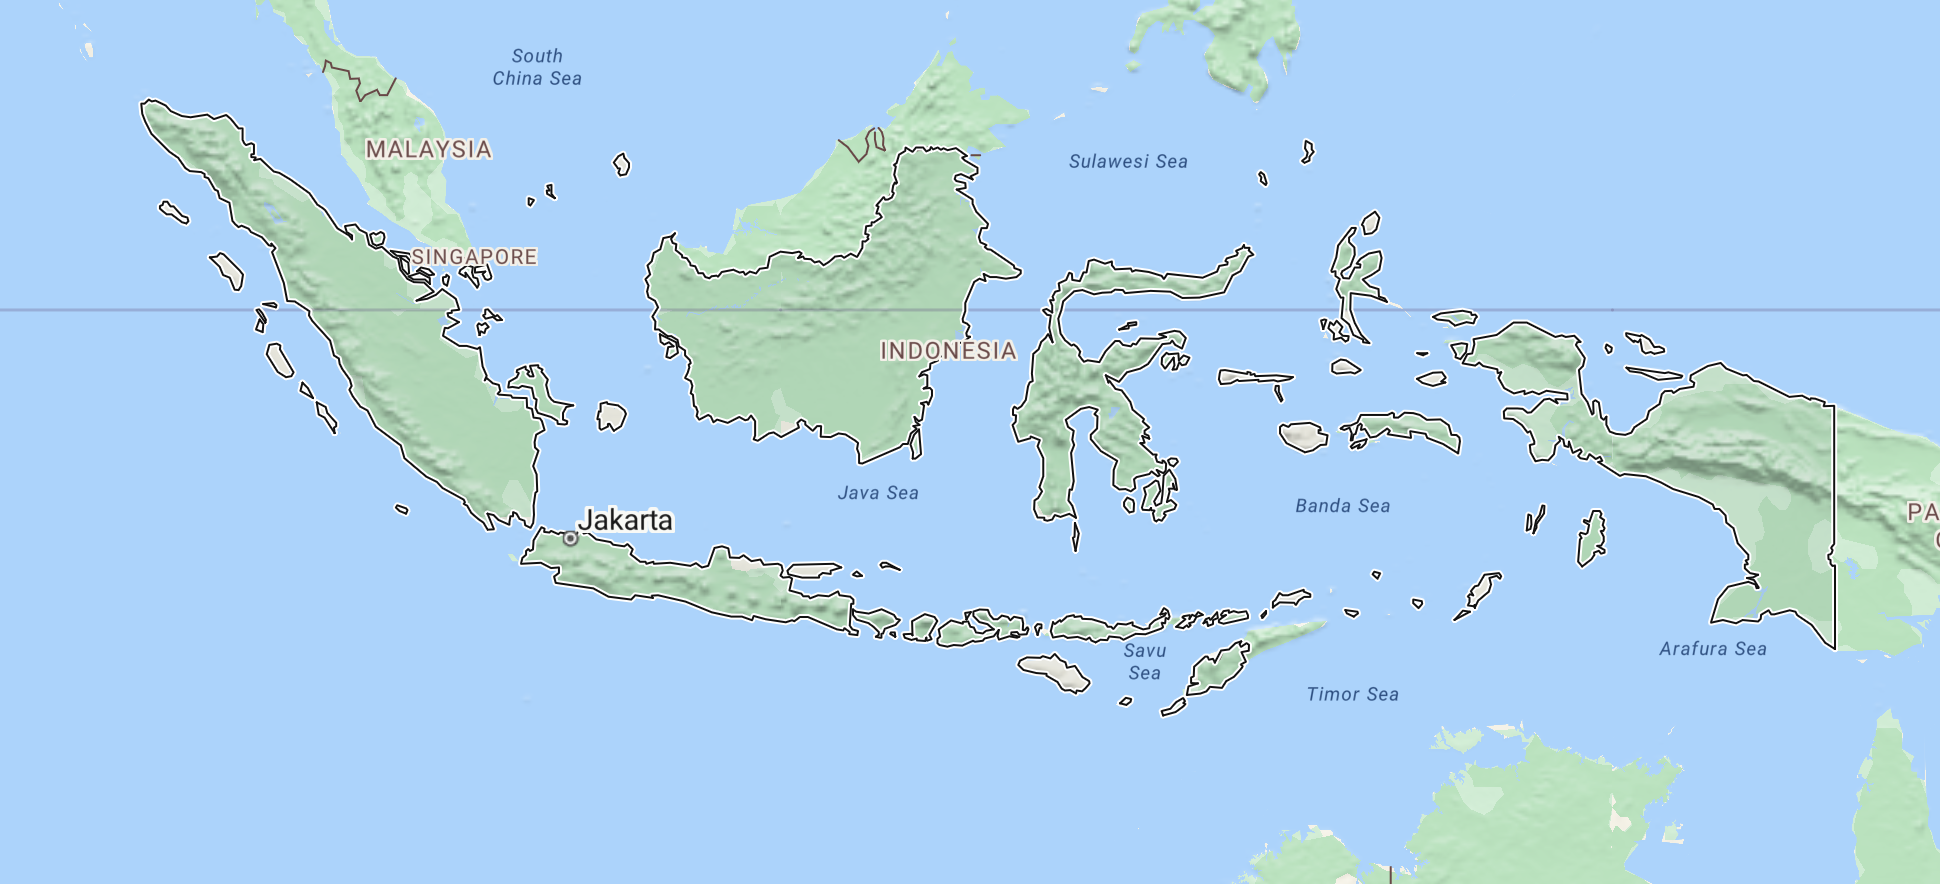
\includegraphics[width=\textwidth]{../images/indonesia}};
\pause
\draw[thick, draw=none, fill=white, fill opacity=0.65] (-2.22, -0.54) -- (1.05, -2.45) -- (1.05, 2.45) -- cycle;
\draw[thick, red] (-2.22, -0.54) -- (1.05, -2.45);
\draw[thick, red] (-2.22, -0.54) -- (1.05, 2.45);
\draw[thick, red, fill=white] (-2.22, -0.54) circle (0.08);
\draw[thick, red, fill=white] (1.05, -2.45) -- (1.05, 2.45) -- (6.05, 2.45) -- (6.05, -2.45) -- cycle;
\node at (3.55, 0) {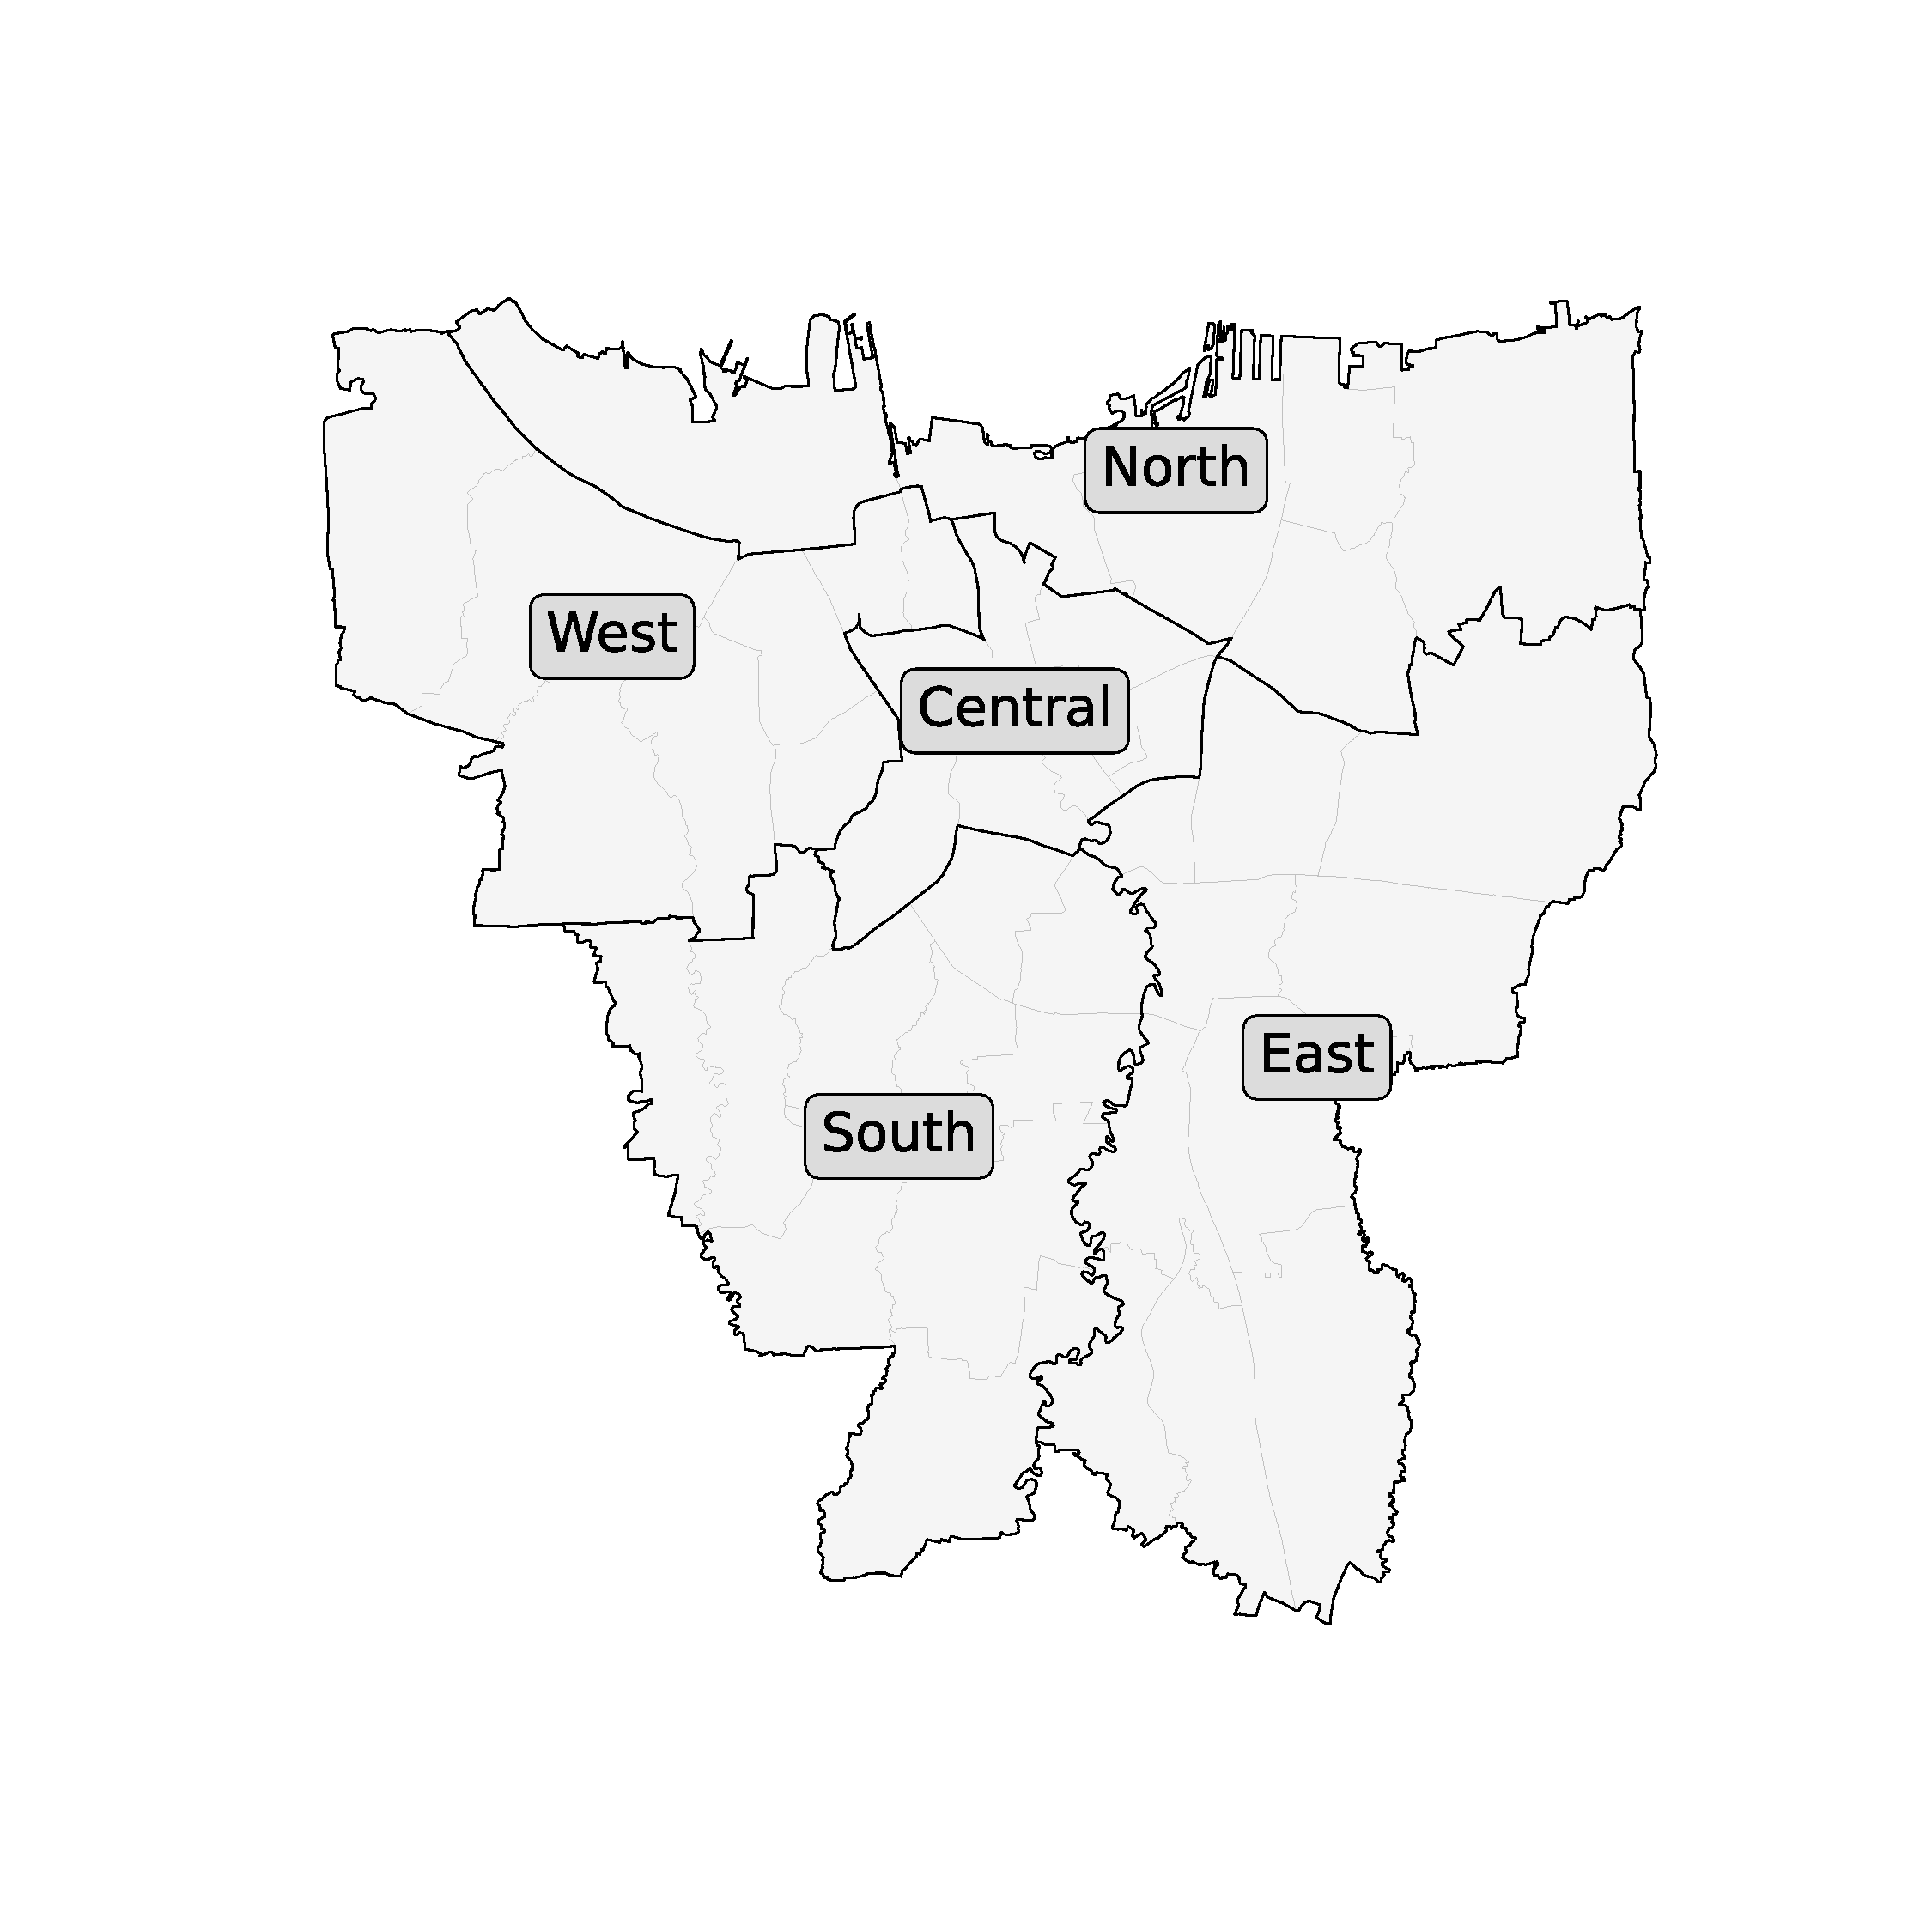
\includegraphics[width=0.4\textwidth]{../images/jakarta_region_names}};
\pause
\node[draw=red, very thick, inner sep=0cm] at (-2.62, 0) {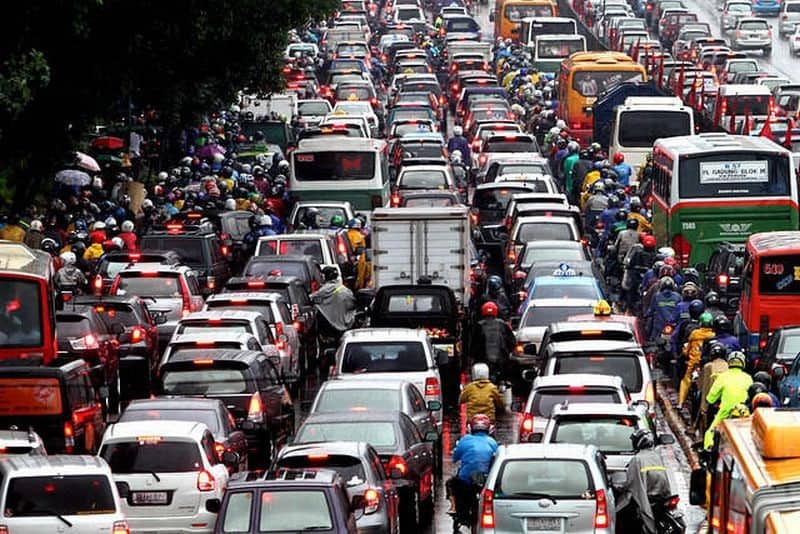
\includegraphics[width=0.6775\textwidth]{../images/jakarta_traffic}};
% \pause
% \draw[thick, red, fill=white] (1.05, -2.45) -- (1.05, 2.45) -- (6.05, 2.45) -- (6.05, -2.45) -- cycle;
% \node at (2.55, 1) {
\includegraphics[width=1.8cm]{../images/ambulans118}};
% \node at (2.55, -1) {
\includegraphics[width=1.8cm]{../cflogo.pdf}};
% \node at (4.55, 1) {
\includegraphics[width=1.8cm]{../images/ambulans119}};
% \node at (4.55, -1) {
\includegraphics[width=1.8cm]{../images/gcrf}};
\end{tikzpicture}%
}
\end{frame}


\begin{frame}
\frametitle{The Problem}
\Wider[4em]{
\resizebox{\textwidth}{!}{%
\begin{tikzpicture}
\node at (0, 0)  {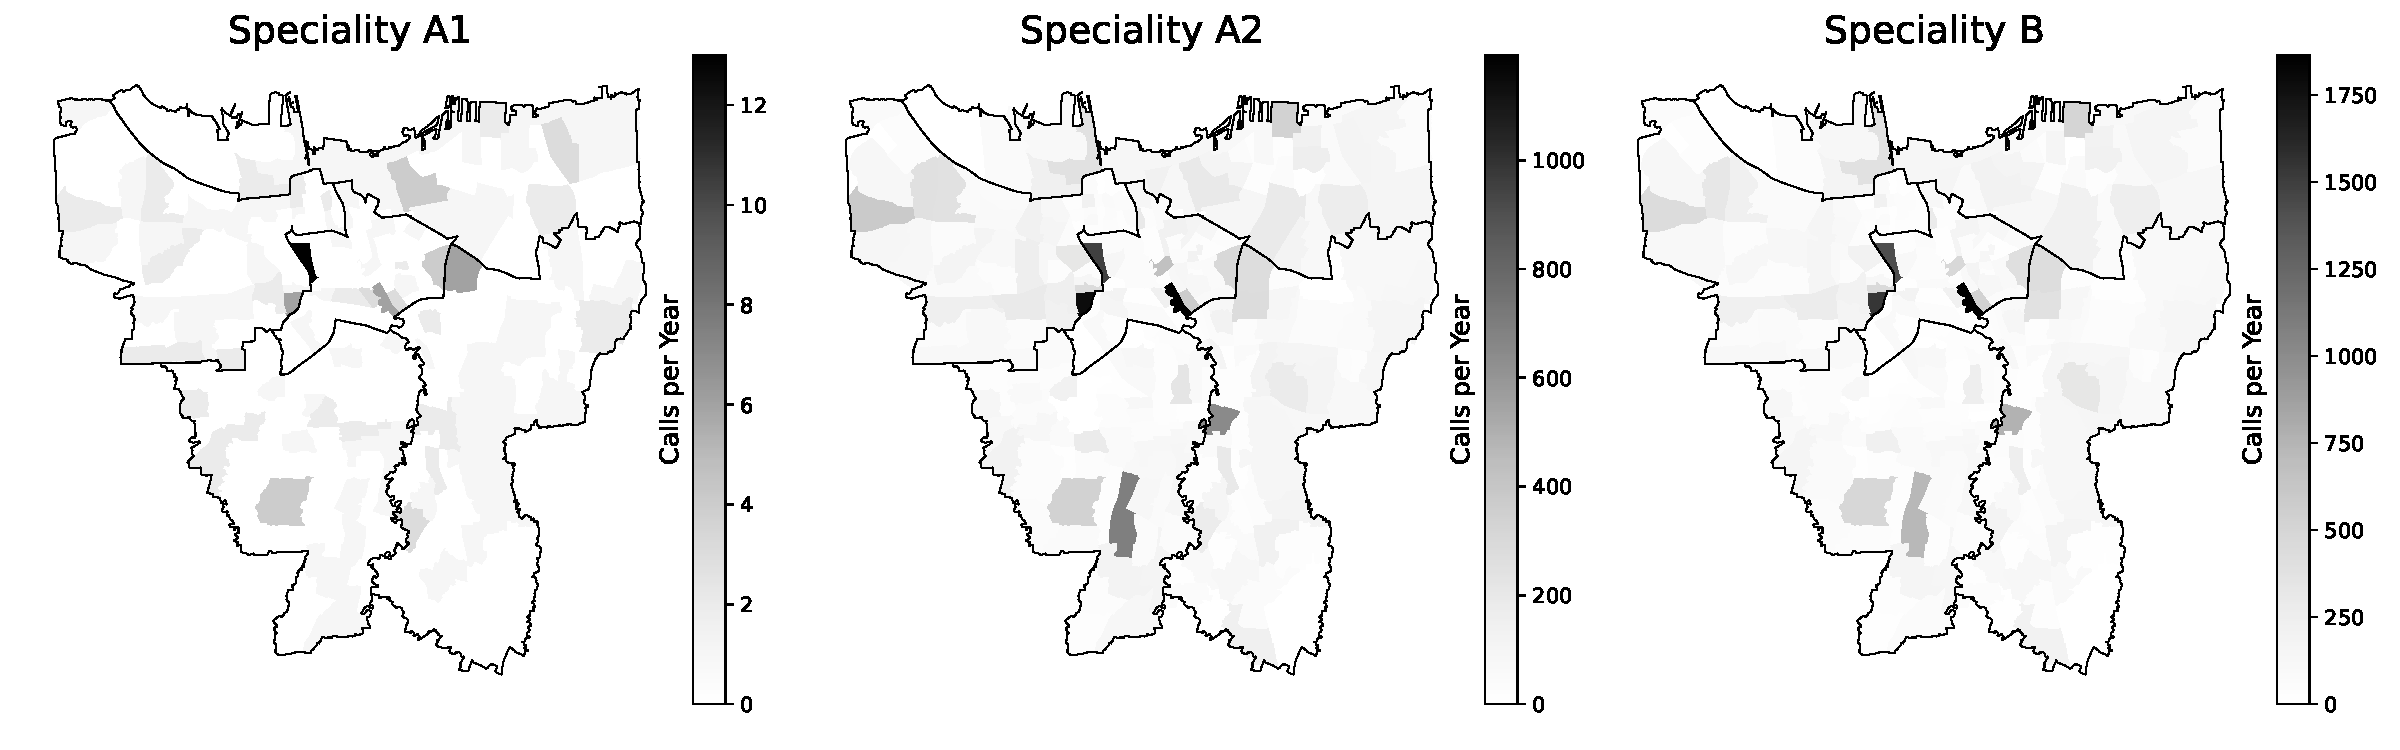
\includegraphics[width=1.08\textwidth]{../images/yearly_demand}};
\pause
\node at (-3.27, 0) {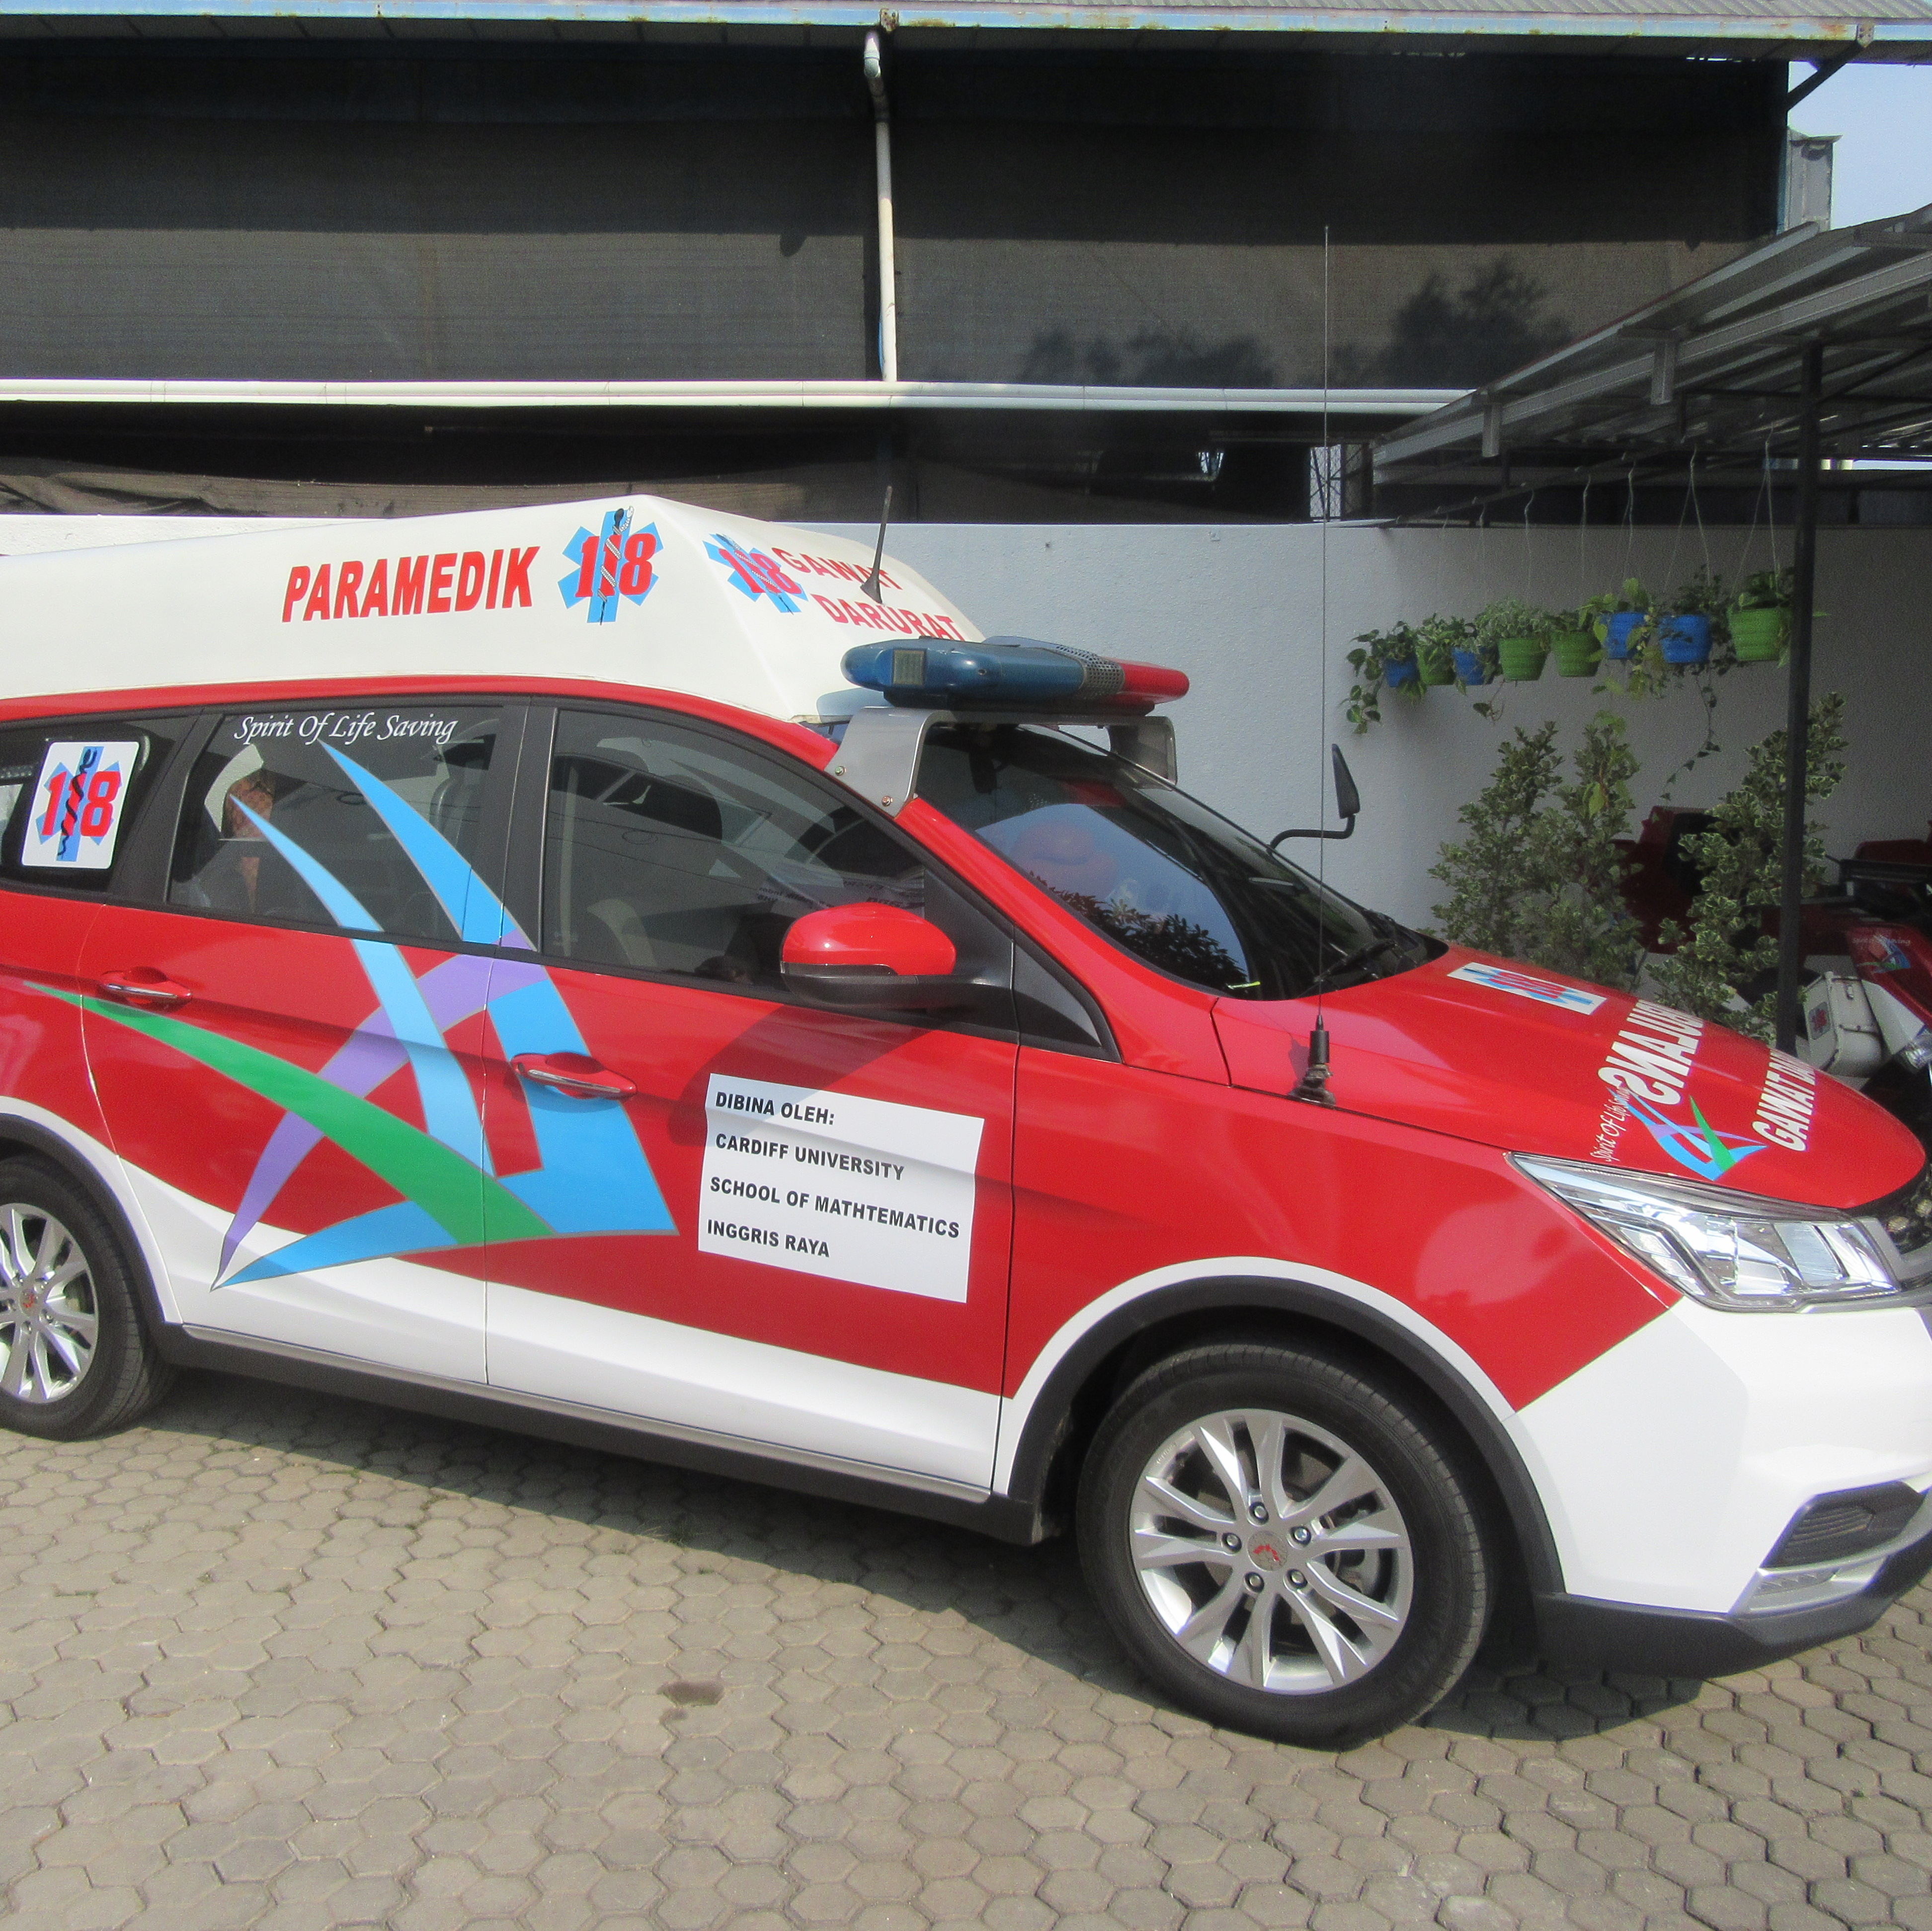
\includegraphics[width=0.53\textwidth]{../images/EA_photo}};
\node[align=center, text=white, fill=black, fill opacity=0.3, text opacity=1, rounded corners] at (-3.27, 2.3) {\textbf{Primary Vehicle}\\\small{Emergency Ambulance (EA)}};
\node at (3.27, 0) {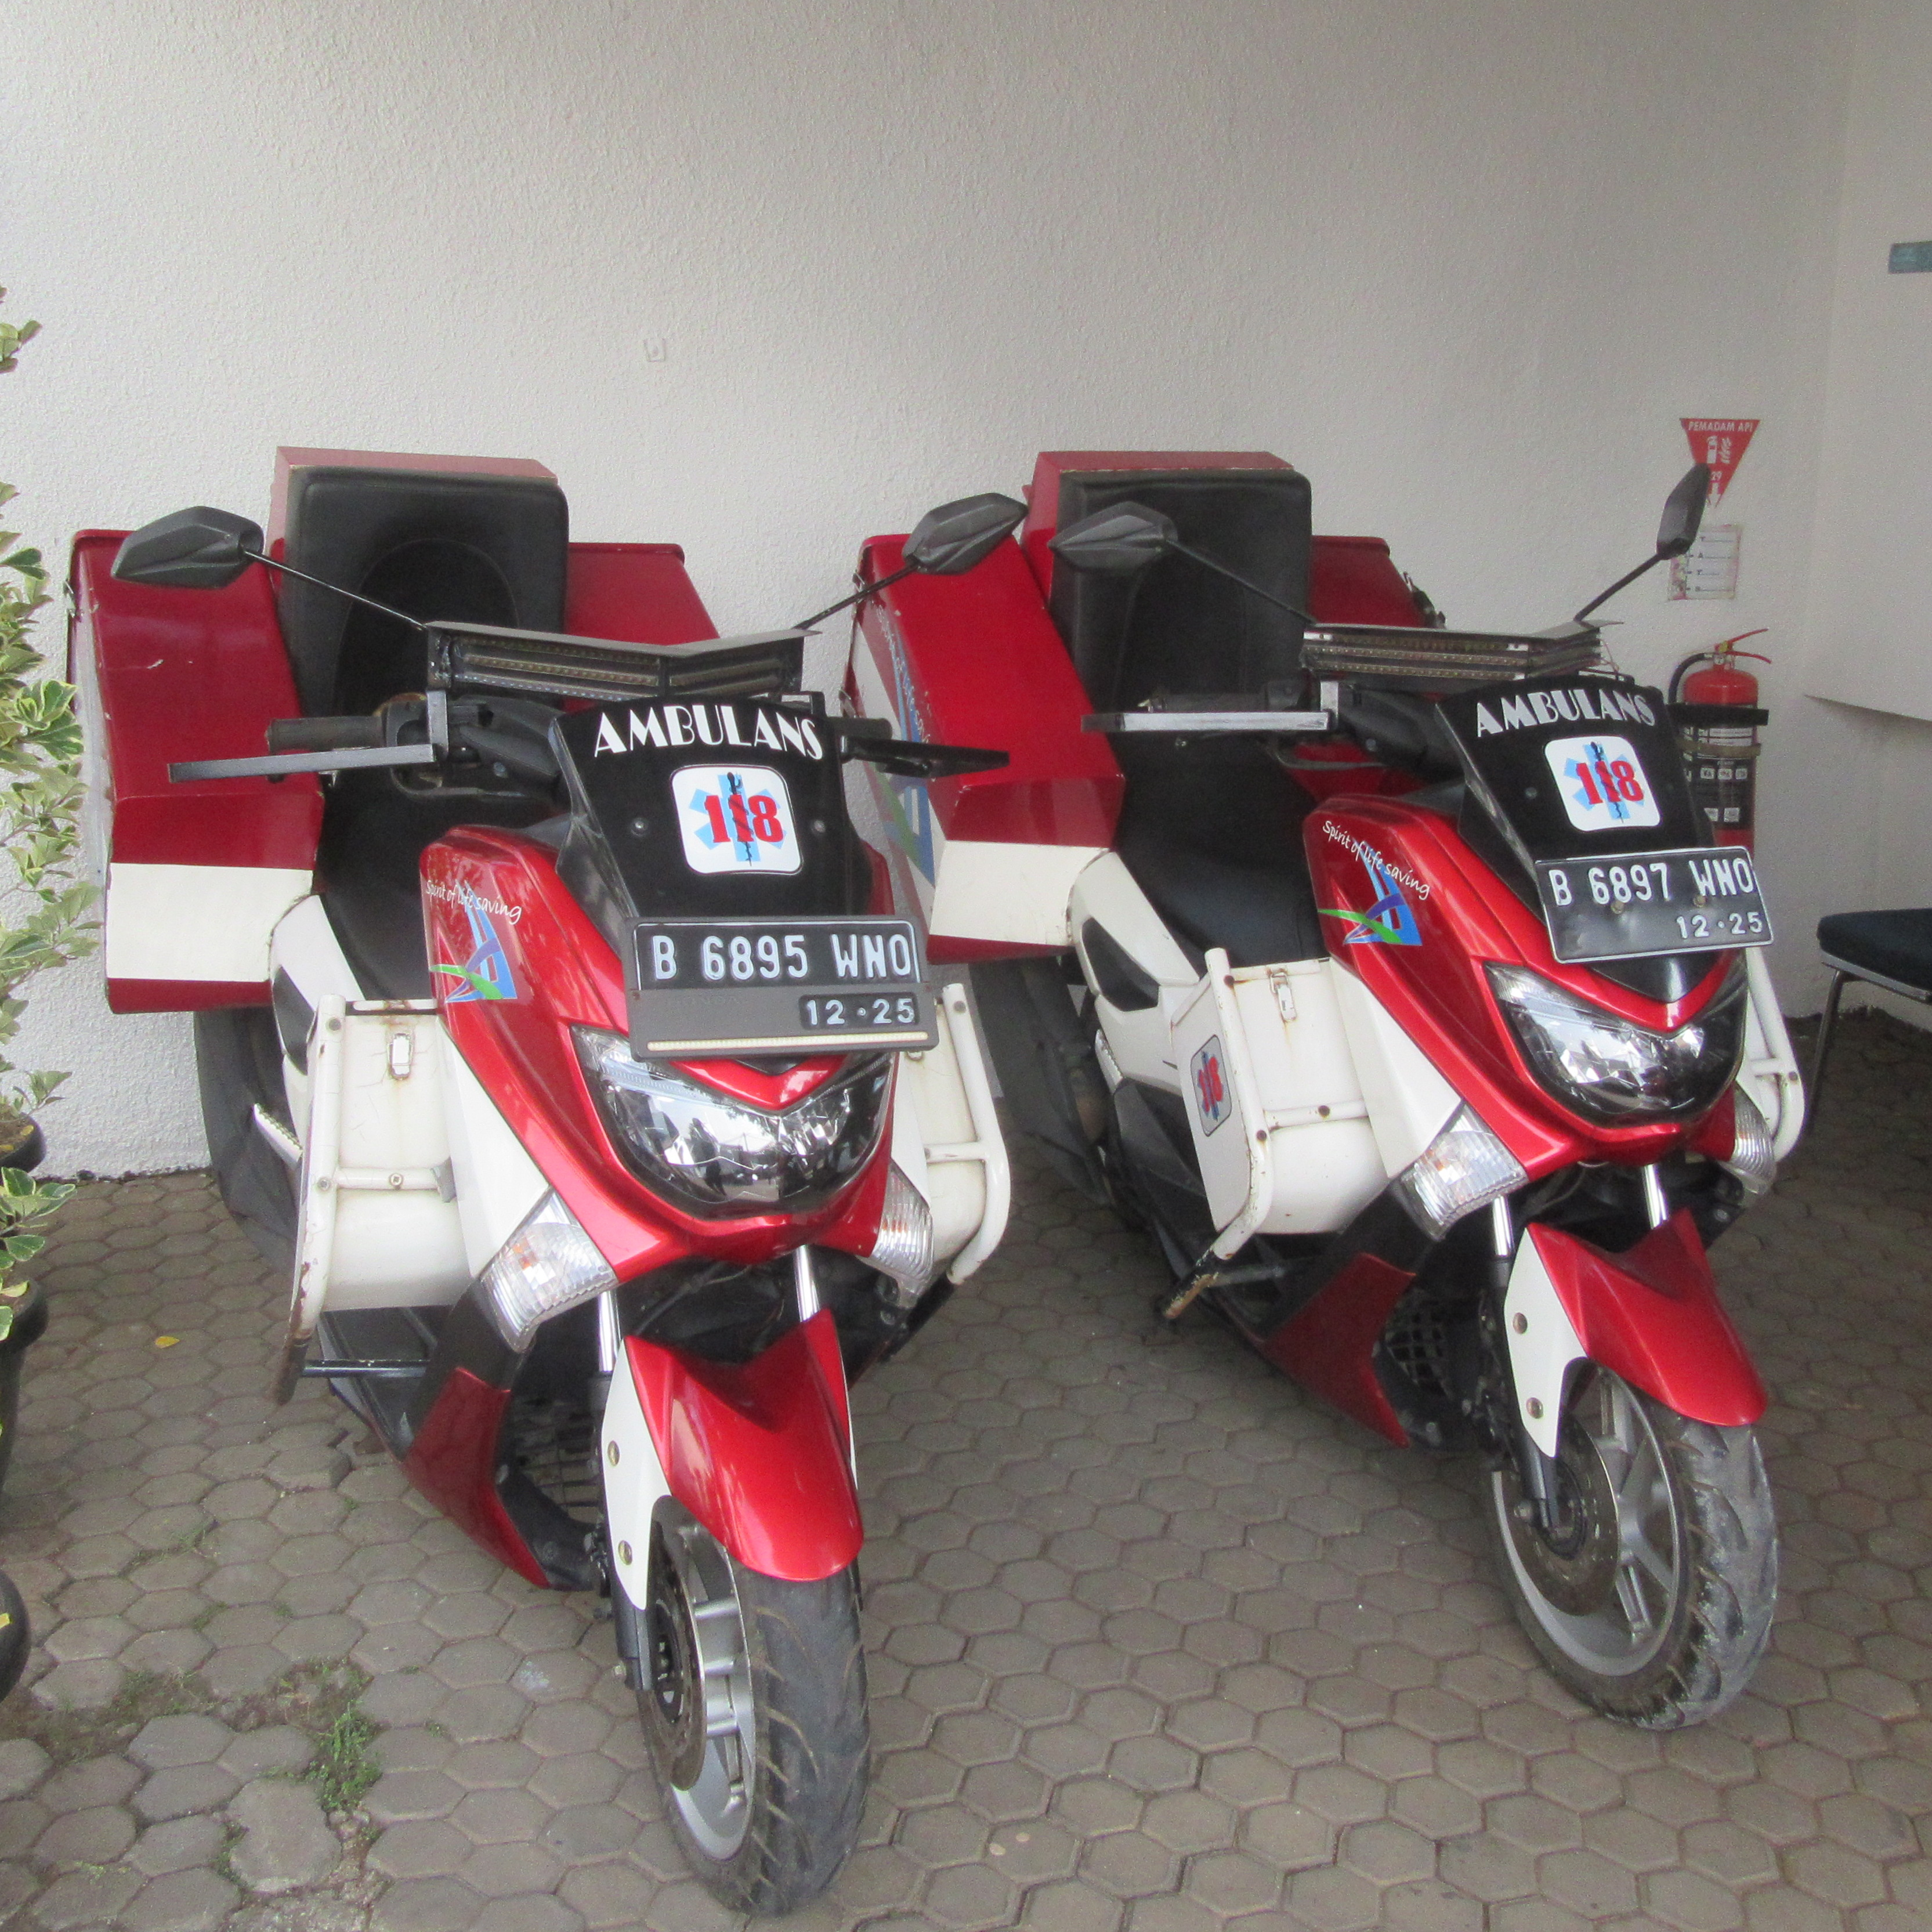
\includegraphics[width=0.53\textwidth]{../images/RRV_photo}};
\node[align=center, text=white, fill=black, fill opacity=0.3, text opacity=1, rounded corners] at (3.27, 2.3) {\textbf{Secondary Vehicle}\\\small{Rapid Response Vehicle (RRV)}};
\pause
\draw[draw=none, fill=white] (-7, -4) rectangle (7, 4);
\node at (0, 0)  {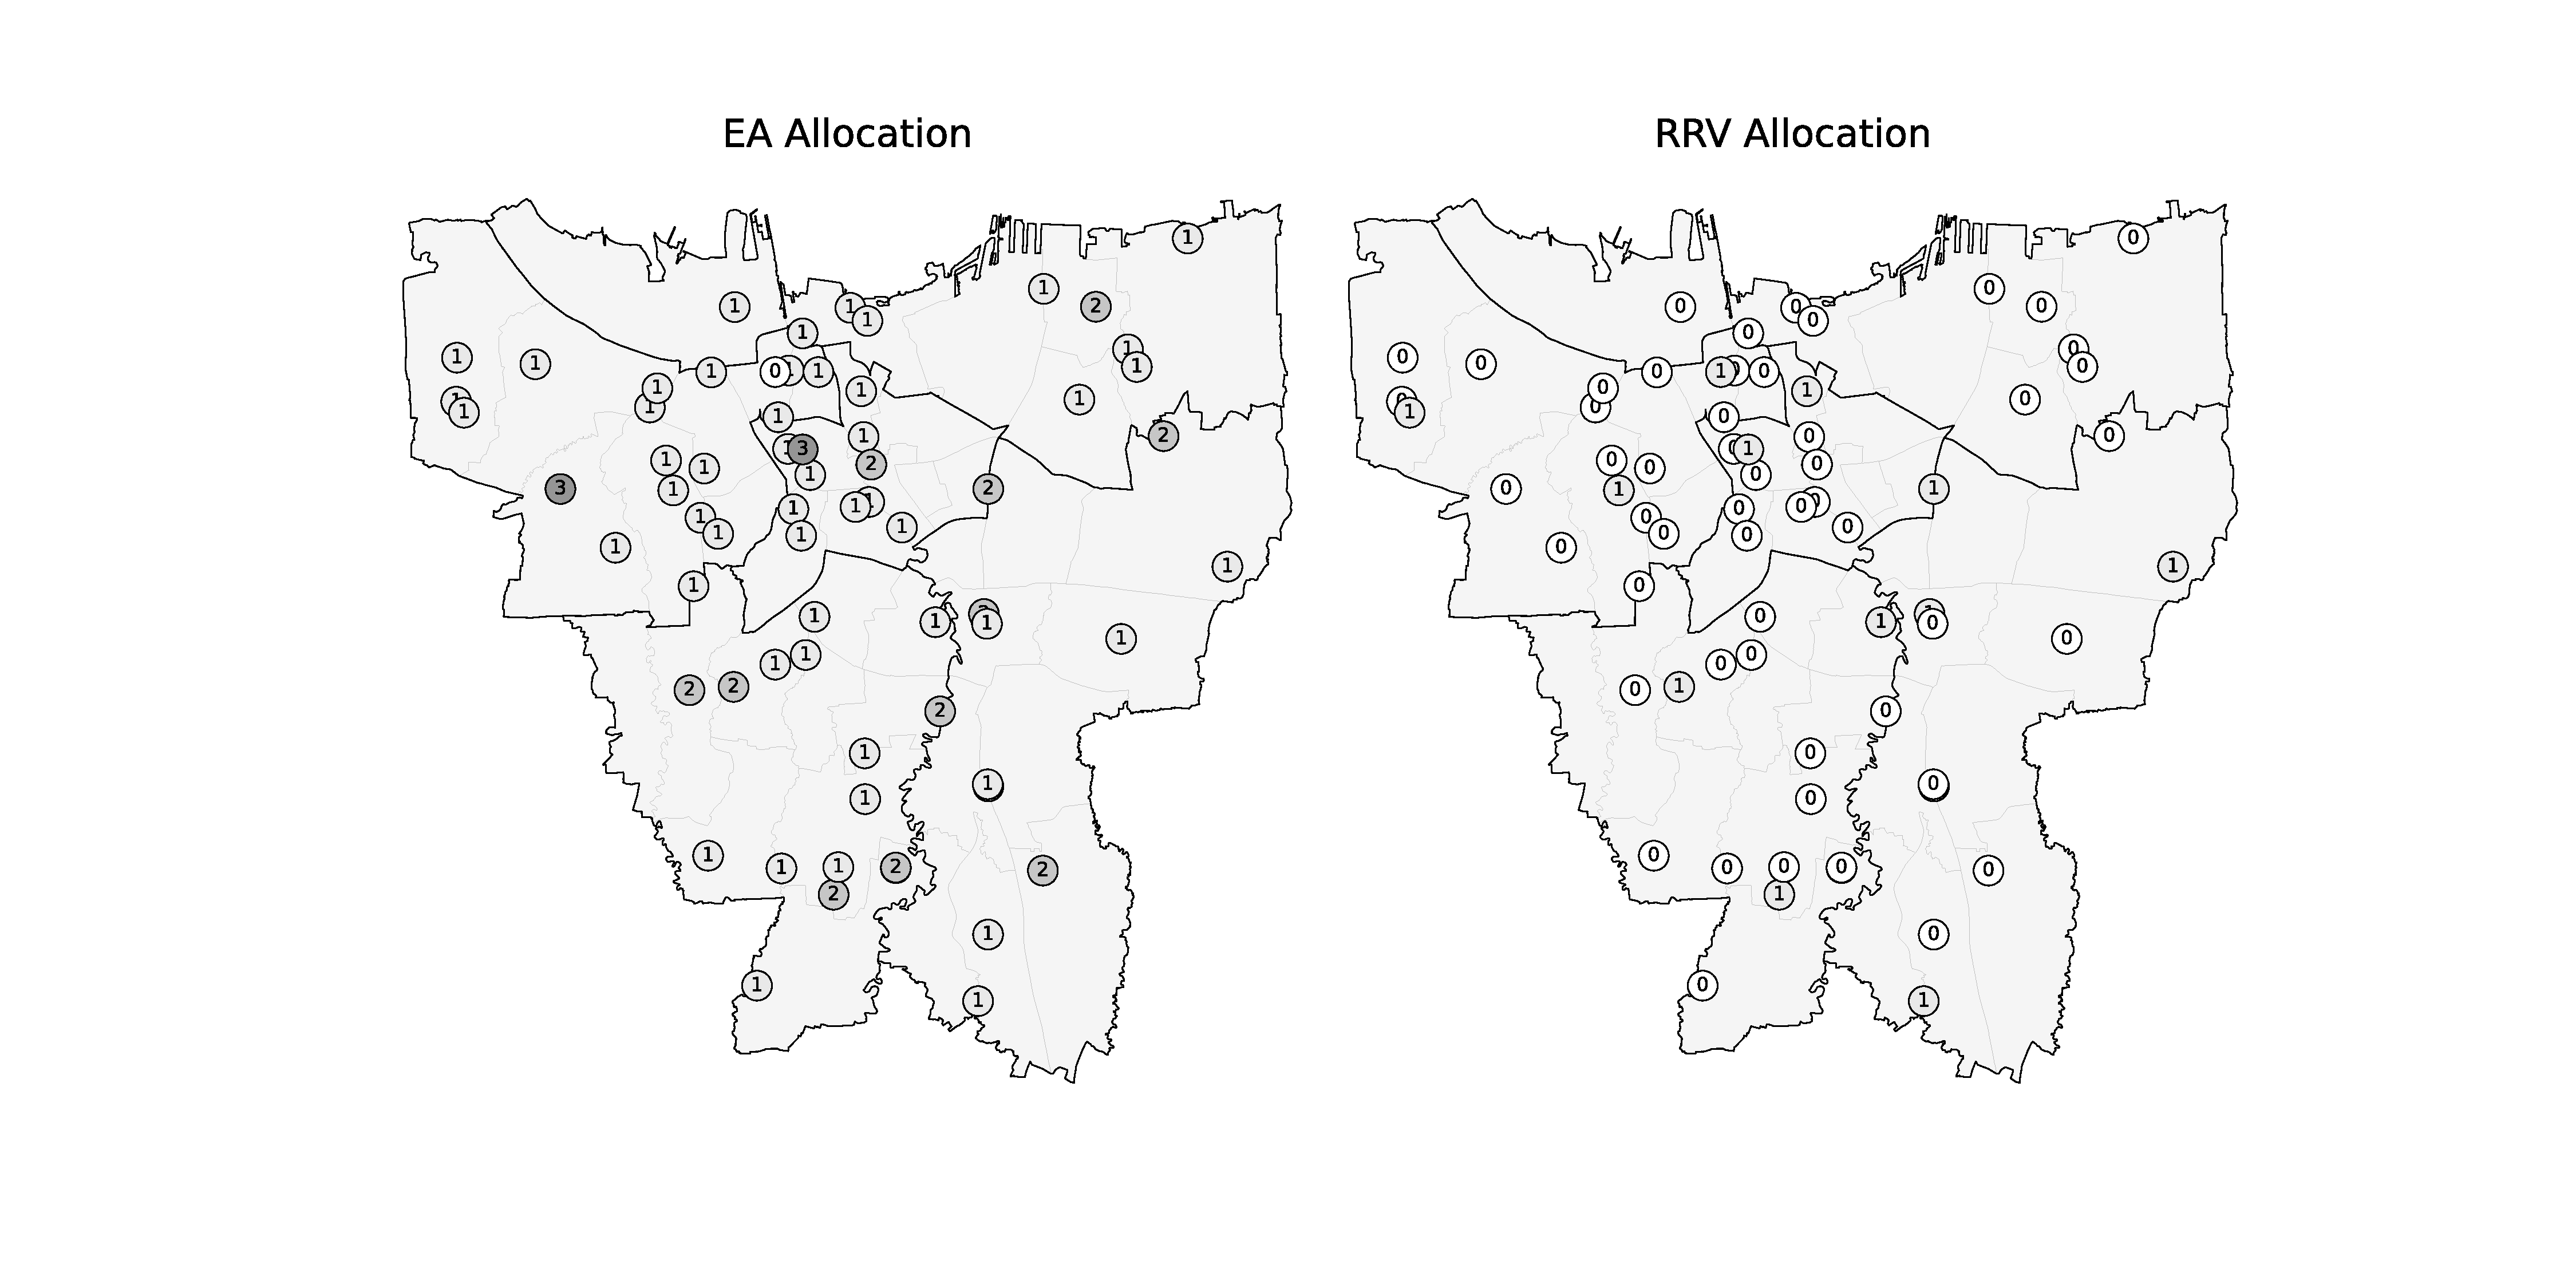
\includegraphics[width=\textwidth]{../images/map_current}};
\end{tikzpicture}%
}%
}
\end{frame}


\begin{frame}
\frametitle{Survival Functions}
\resizebox{\textwidth}{!}{%
\begin{tikzpicture}
\node at (-2.5, 0) {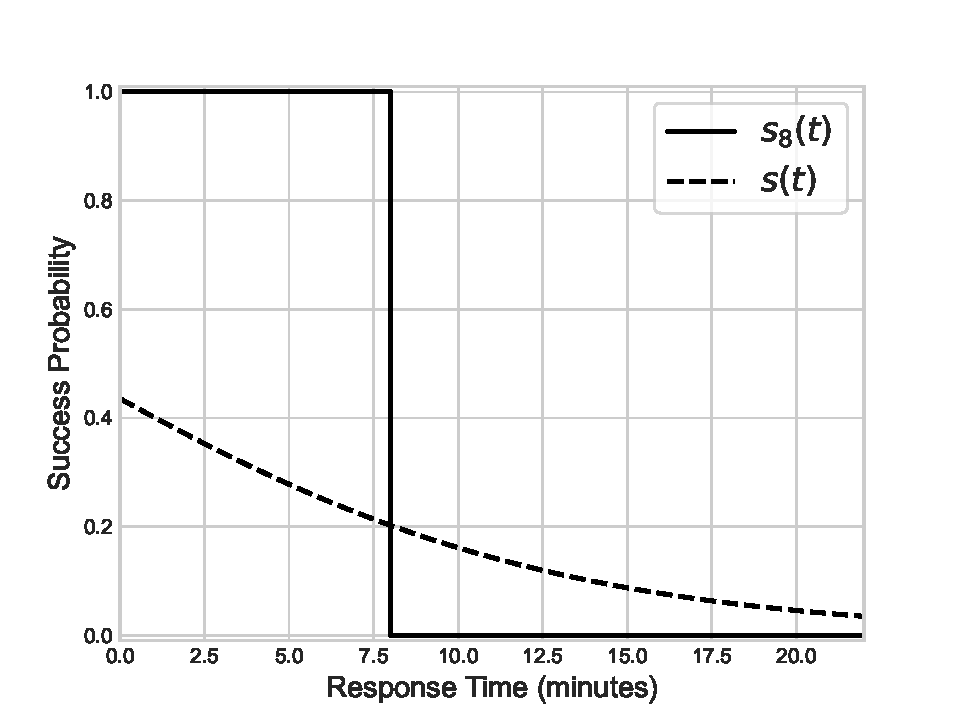
\includegraphics[width=0.5\textwidth]{../images/Survival_Function}};
\node at (2.5, 1) {$s(t) = \left(1 + e^{0.26+0.139t}\right)^{-1}$};
\node at (2.5, -1) {$ s_L(t) = \begin{cases} 1 \text{ if } 0\leq t \leq L \\ 0 \text{ if } t > L \end{cases}$};
\end{tikzpicture}%
}
\end{frame}

\begin{frame}
\frametitle{Plan: Optimisation \& Simulation}
\resizebox{\textwidth}{!}{%
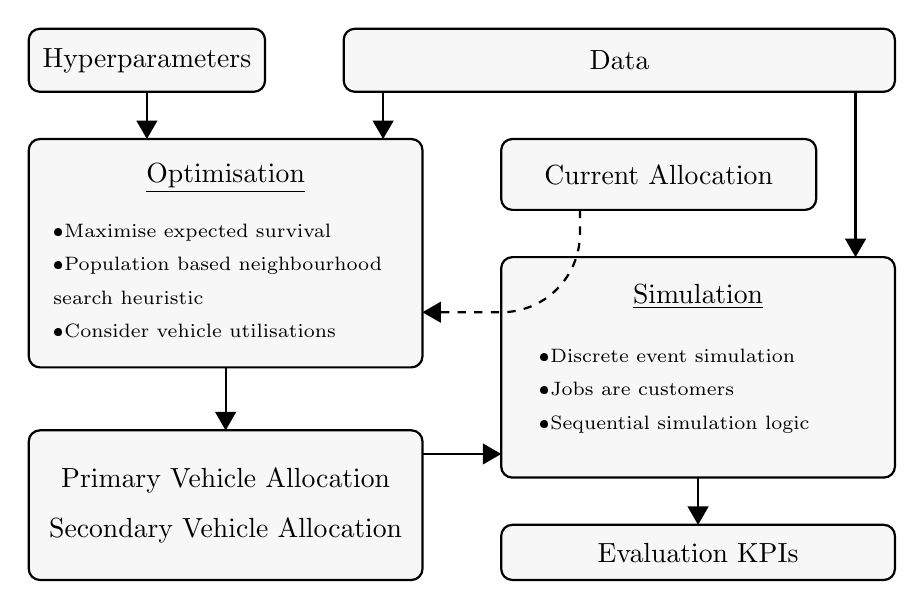
\begin{tikzpicture}
\draw[thick, rounded corners, fill=black!3] (0, 2.7) rectangle (5, 5.6); % Optimisation
\node at (2.5, 5.1) {\underline{Optimisation}};
\node[align=left] at (2.4, 3.8) {\scriptsize{\textbullet Maximise expected survival}\\\scriptsize{\textbullet Population based neighbourhood}\\\scriptsize{search heuristic}\\\scriptsize{\textbullet Consider vehicle utilisations}};
% \only<1,3->{
  \draw[thick, rounded corners, fill=black!3] (6, 1.3) rectangle (11, 4.1); % Simulation
  \node at (8.5, 3.6) {\underline{Simulation}};
  \node[align=left] at (8.2, 2.4) {\scriptsize{\textbullet Discrete event simulation}\\\scriptsize{\textbullet Jobs are customers}\\\scriptsize{\textbullet Sequential simulation logic}};
% }

% \pause
\draw[thick, rounded corners, fill=black!3] (0, 0) rectangle (5, 1.9); % Allocation
\node at (2.5, 1.266) {Primary Vehicle Allocation};
\node at (2.5, 0.633) {Secondary Vehicle Allocation};
\draw[thick, -triangle 60] (2.5, 2.7) -- (2.5, 1.9);
\draw[thick, rounded corners, fill=black!3] (0, 6.2) rectangle (3, 7); % Hyperparameters
\node at (1.5, 6.6) {Hyperparameters};
\draw[thick, -triangle 60] (1.5, 6.2) -- (1.5, 5.6);
\draw[thick, rounded corners, fill=black!3] (4, 6.2) rectangle (11, 7); % Data
\node at (7.5, 6.6) {Data};
\draw[thick, -triangle 60] (4.5, 6.2) -- (4.5, 5.6);

% \pause
\draw[thick, rounded corners, fill=black!3] (6, 0) rectangle (11, 0.7); % KPIs
\node at (8.5, 0.35) {Evaluation KPIs};
\draw[thick, -triangle 60] (8.5, 1.3) -- (8.5, 0.7);
\draw[thick, -triangle 60] (10.5, 6.2) -- (10.5, 4.1);
\draw[thick, -triangle 60] (5, 1.6) -- (6, 1.6);

% \pause
\draw[thick, rounded corners, fill=black!3] (6, 4.7) rectangle (10, 5.6); % Current allocation
\node at (8, 5.15) {Current Allocation};
\draw [thick, -triangle 60, dashed, rounded corners=10mm] (7, 4.7) -- (7, 3.4) -- (5, 3.4);

\end{tikzpicture}%
}
\end{frame}


\begin{frame}
\frametitle{MESLMHPHF}
\Wider[4em]{
\begin{center}
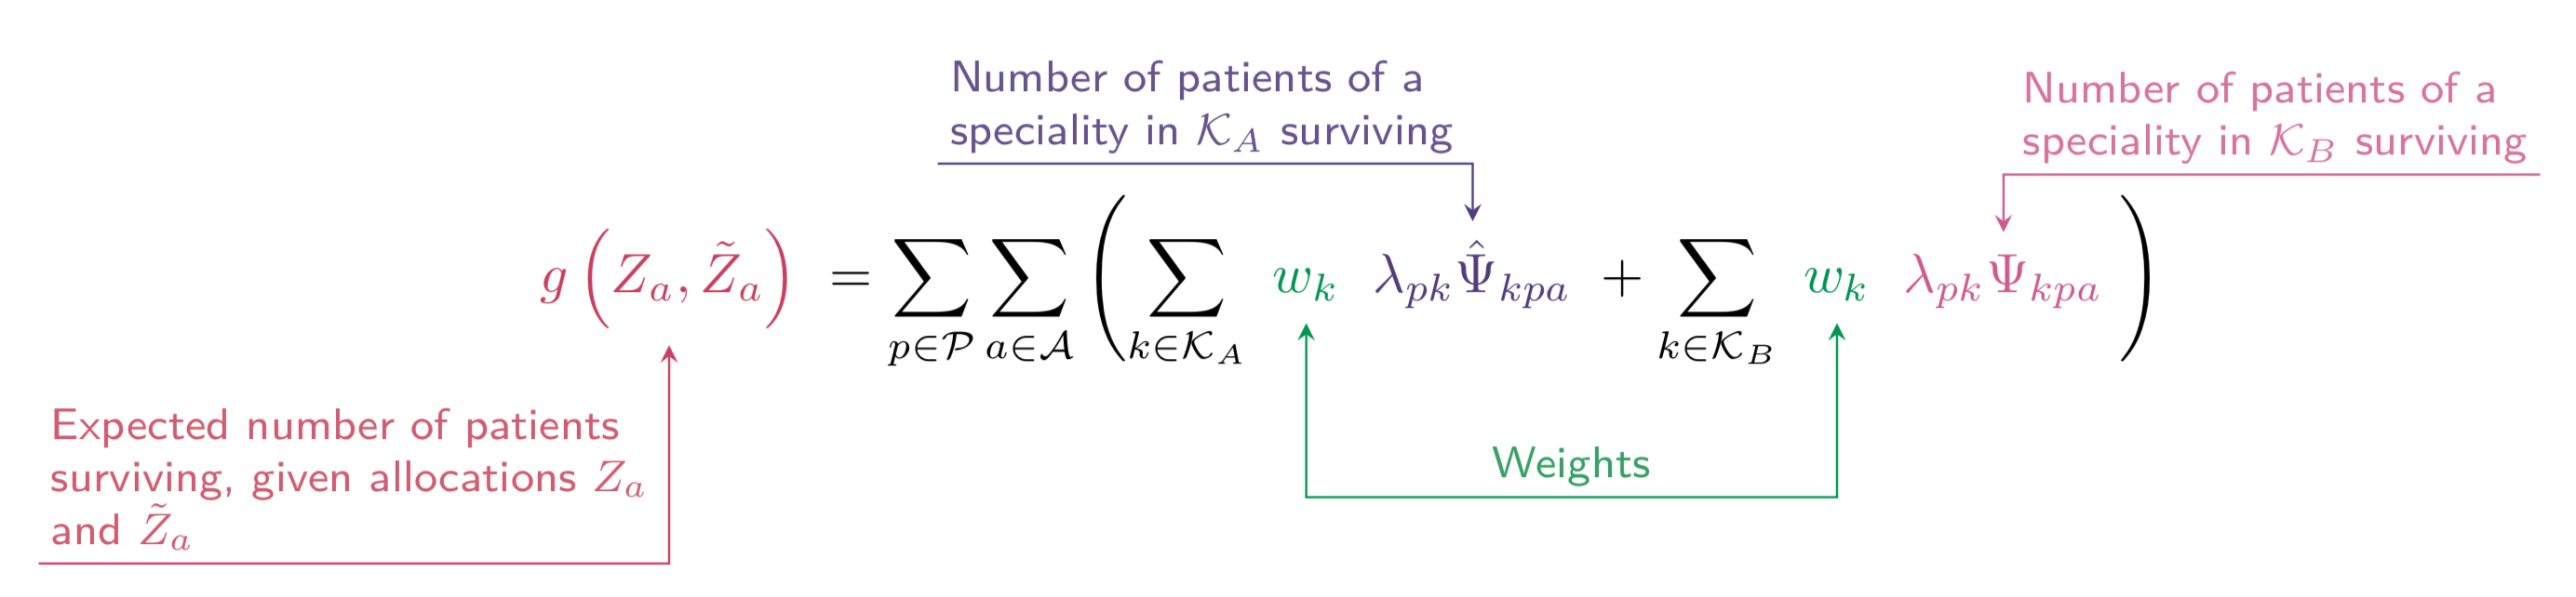
\includegraphics[width=\textwidth]{../images/meslmhphf}
\end{center}%
}
\end{frame}


\begin{frame}
\Wider[4em]{
\begin{center}
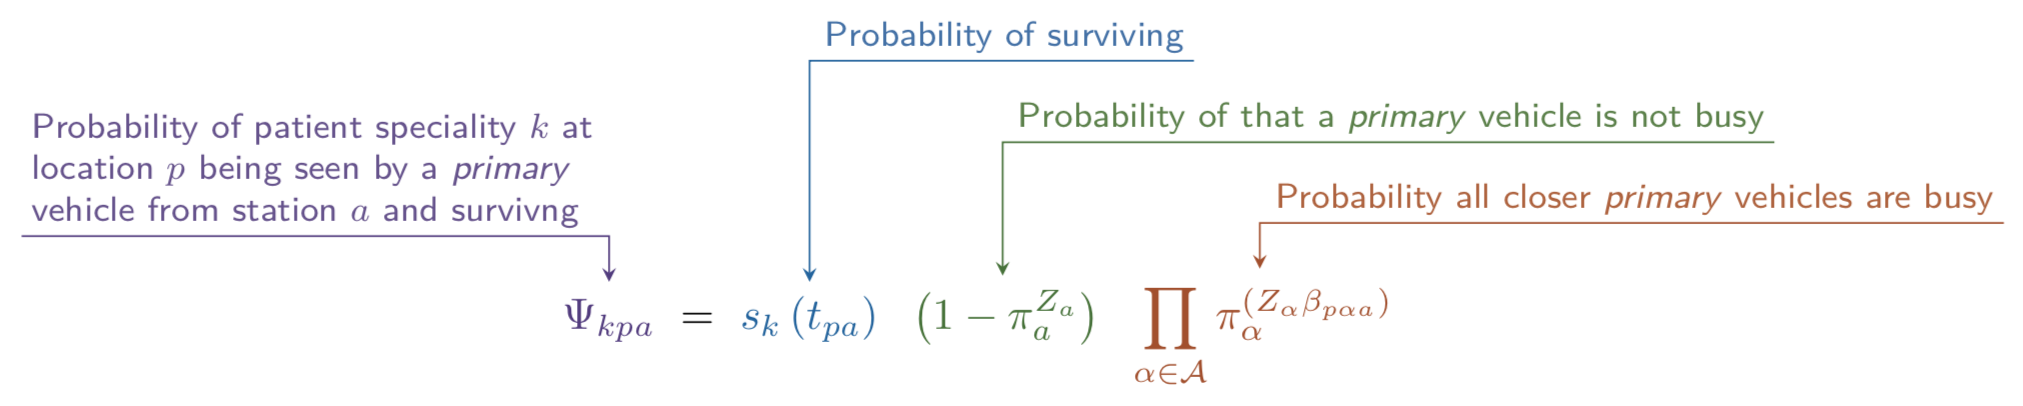
\includegraphics[width=\textwidth]{../images/psi}
\end{center}%
}
\end{frame}

\begin{frame}
\Wider[4em]{
\begin{center}
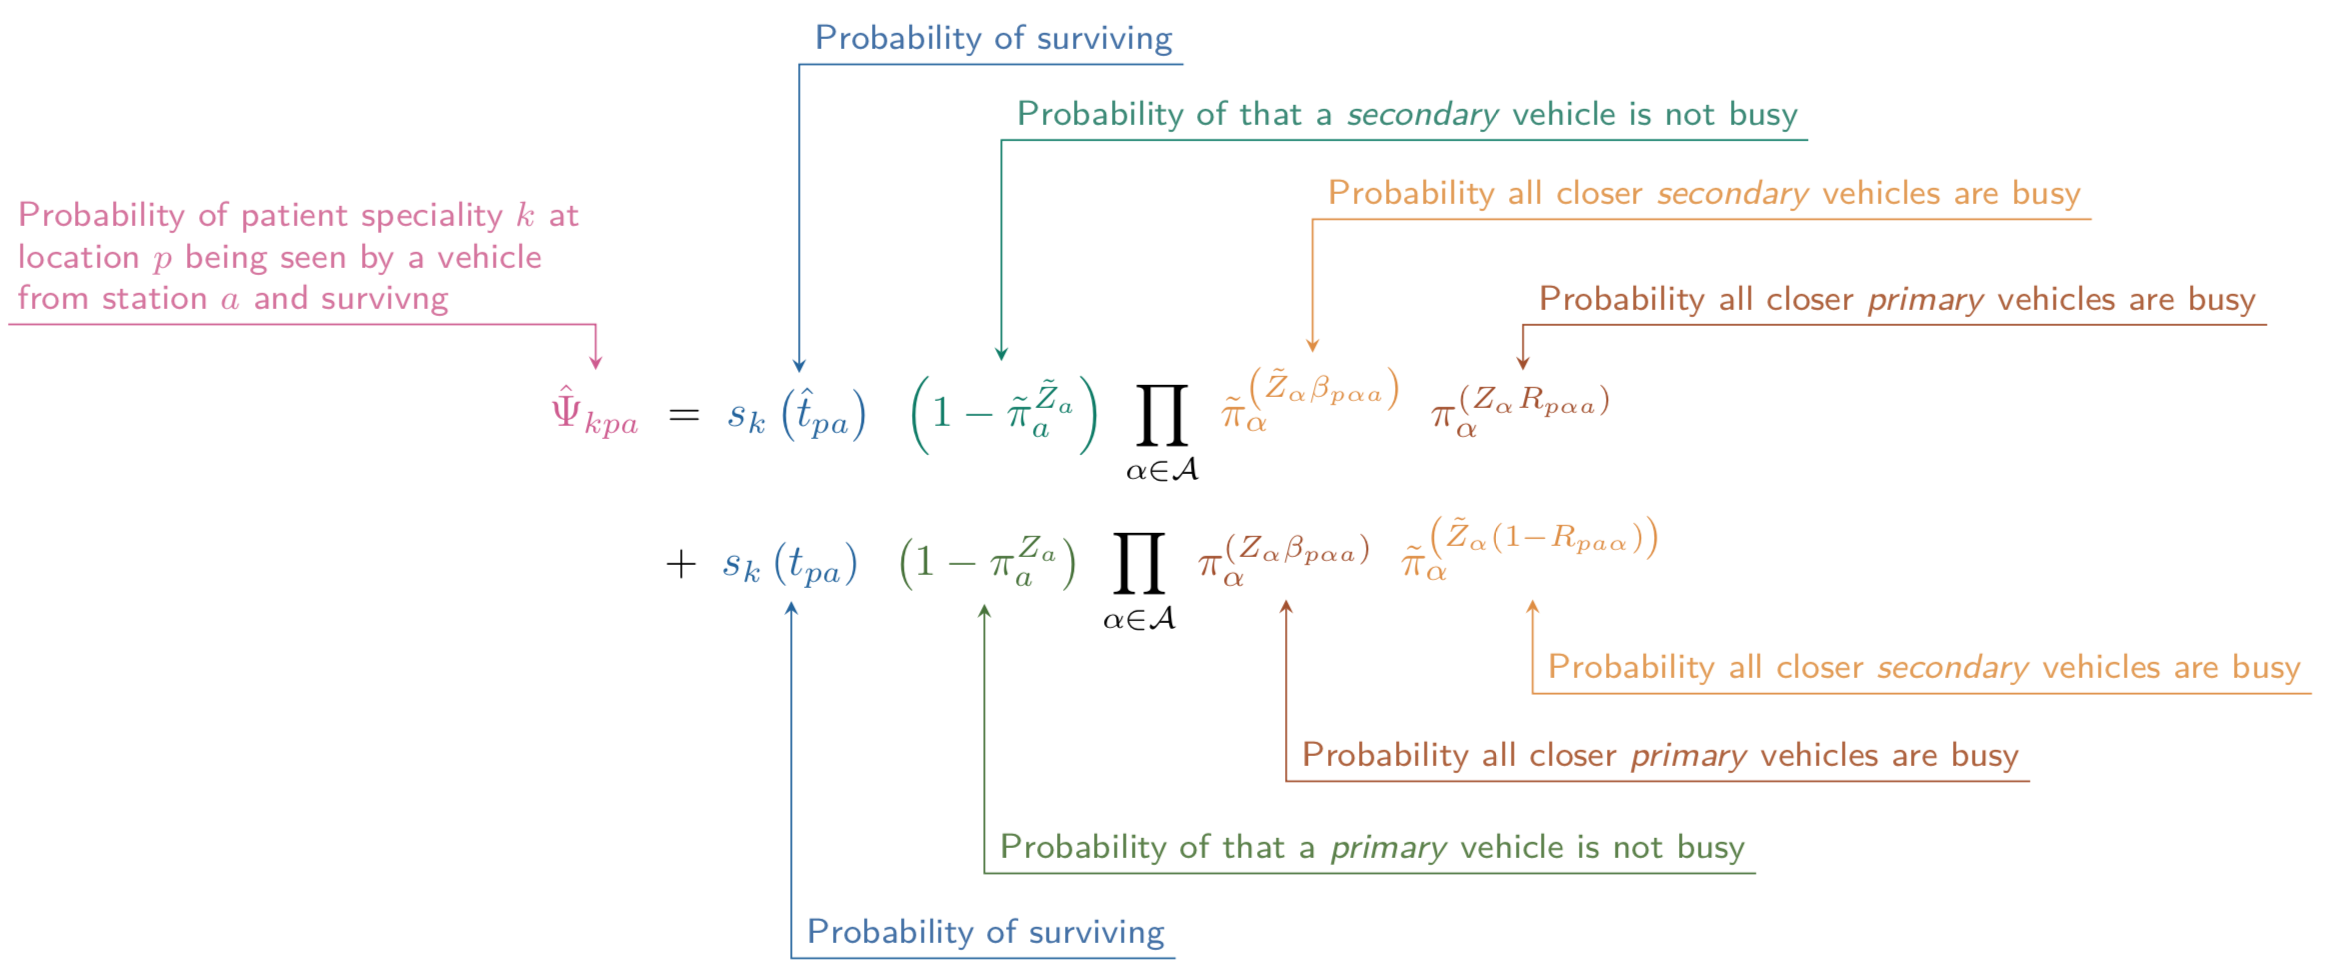
\includegraphics[width=\textwidth]{../images/psi_tilde}
\end{center}%
}
\end{frame}

\begin{frame}
\frametitle{Utilisations}
\begin{center}
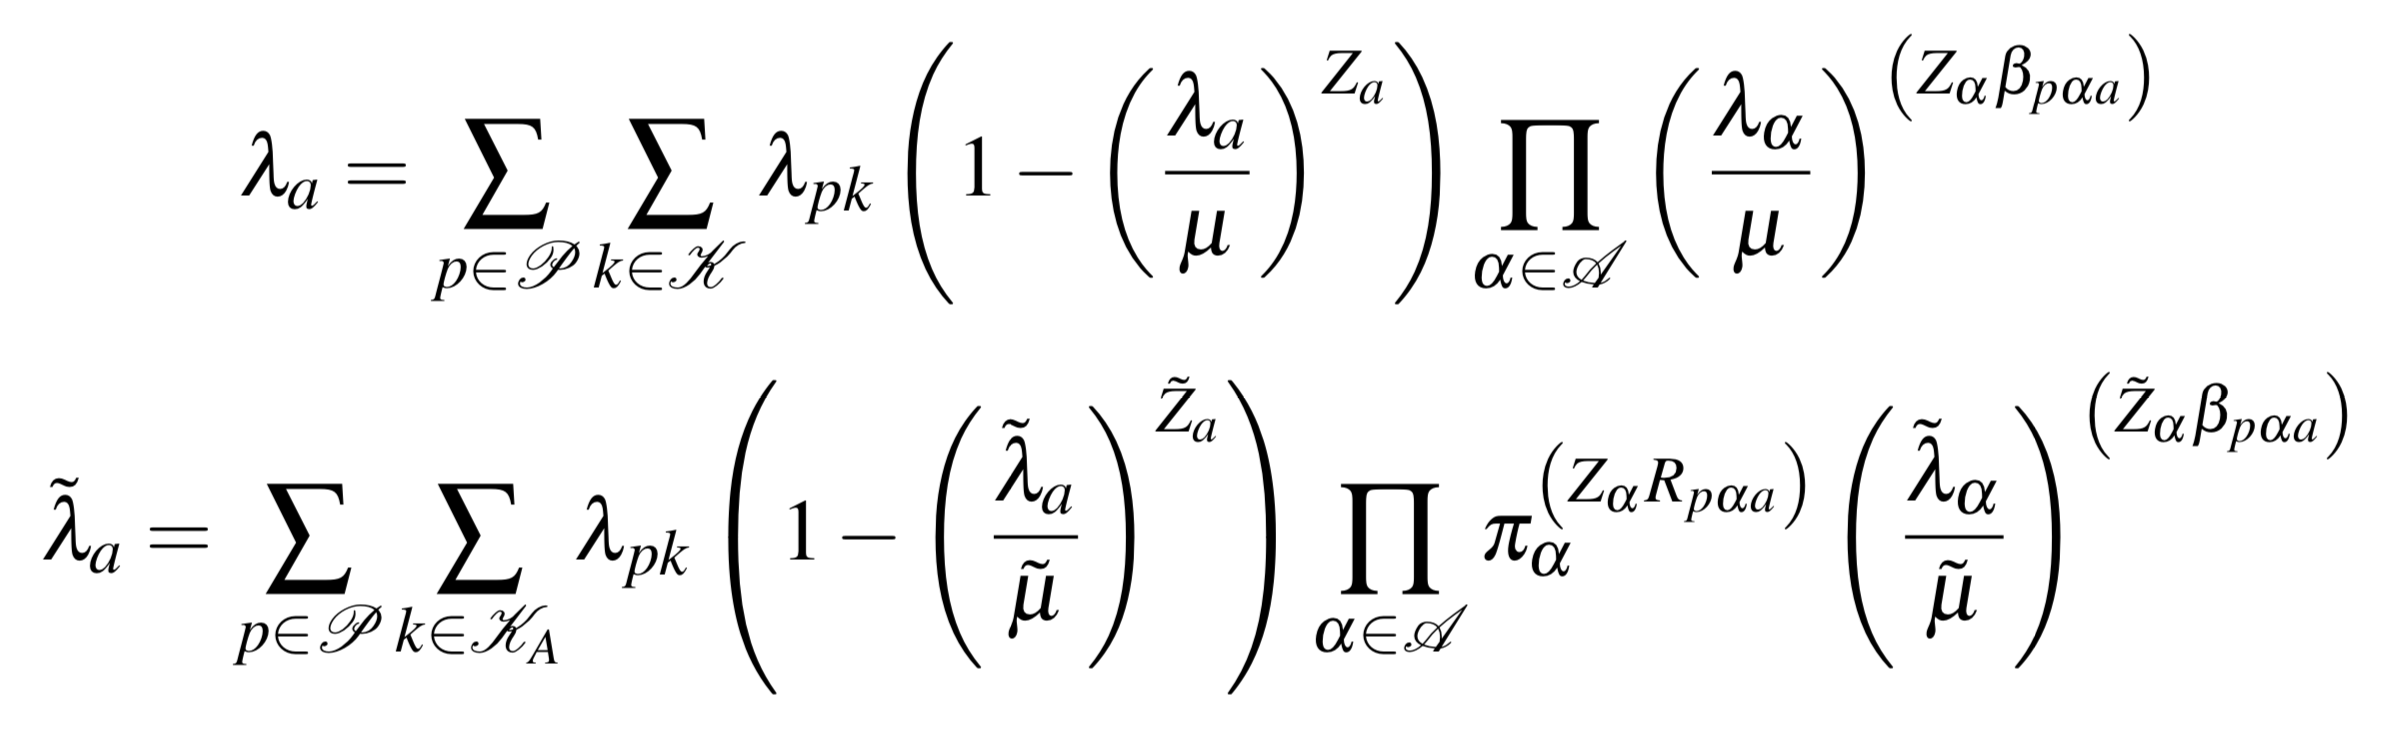
\includegraphics[width=\textwidth]{../images/utilisations}
\end{center}
\end{frame}

\begin{frame}
\frametitle{Heuristic}
\Wider[4em]{
\begin{center}
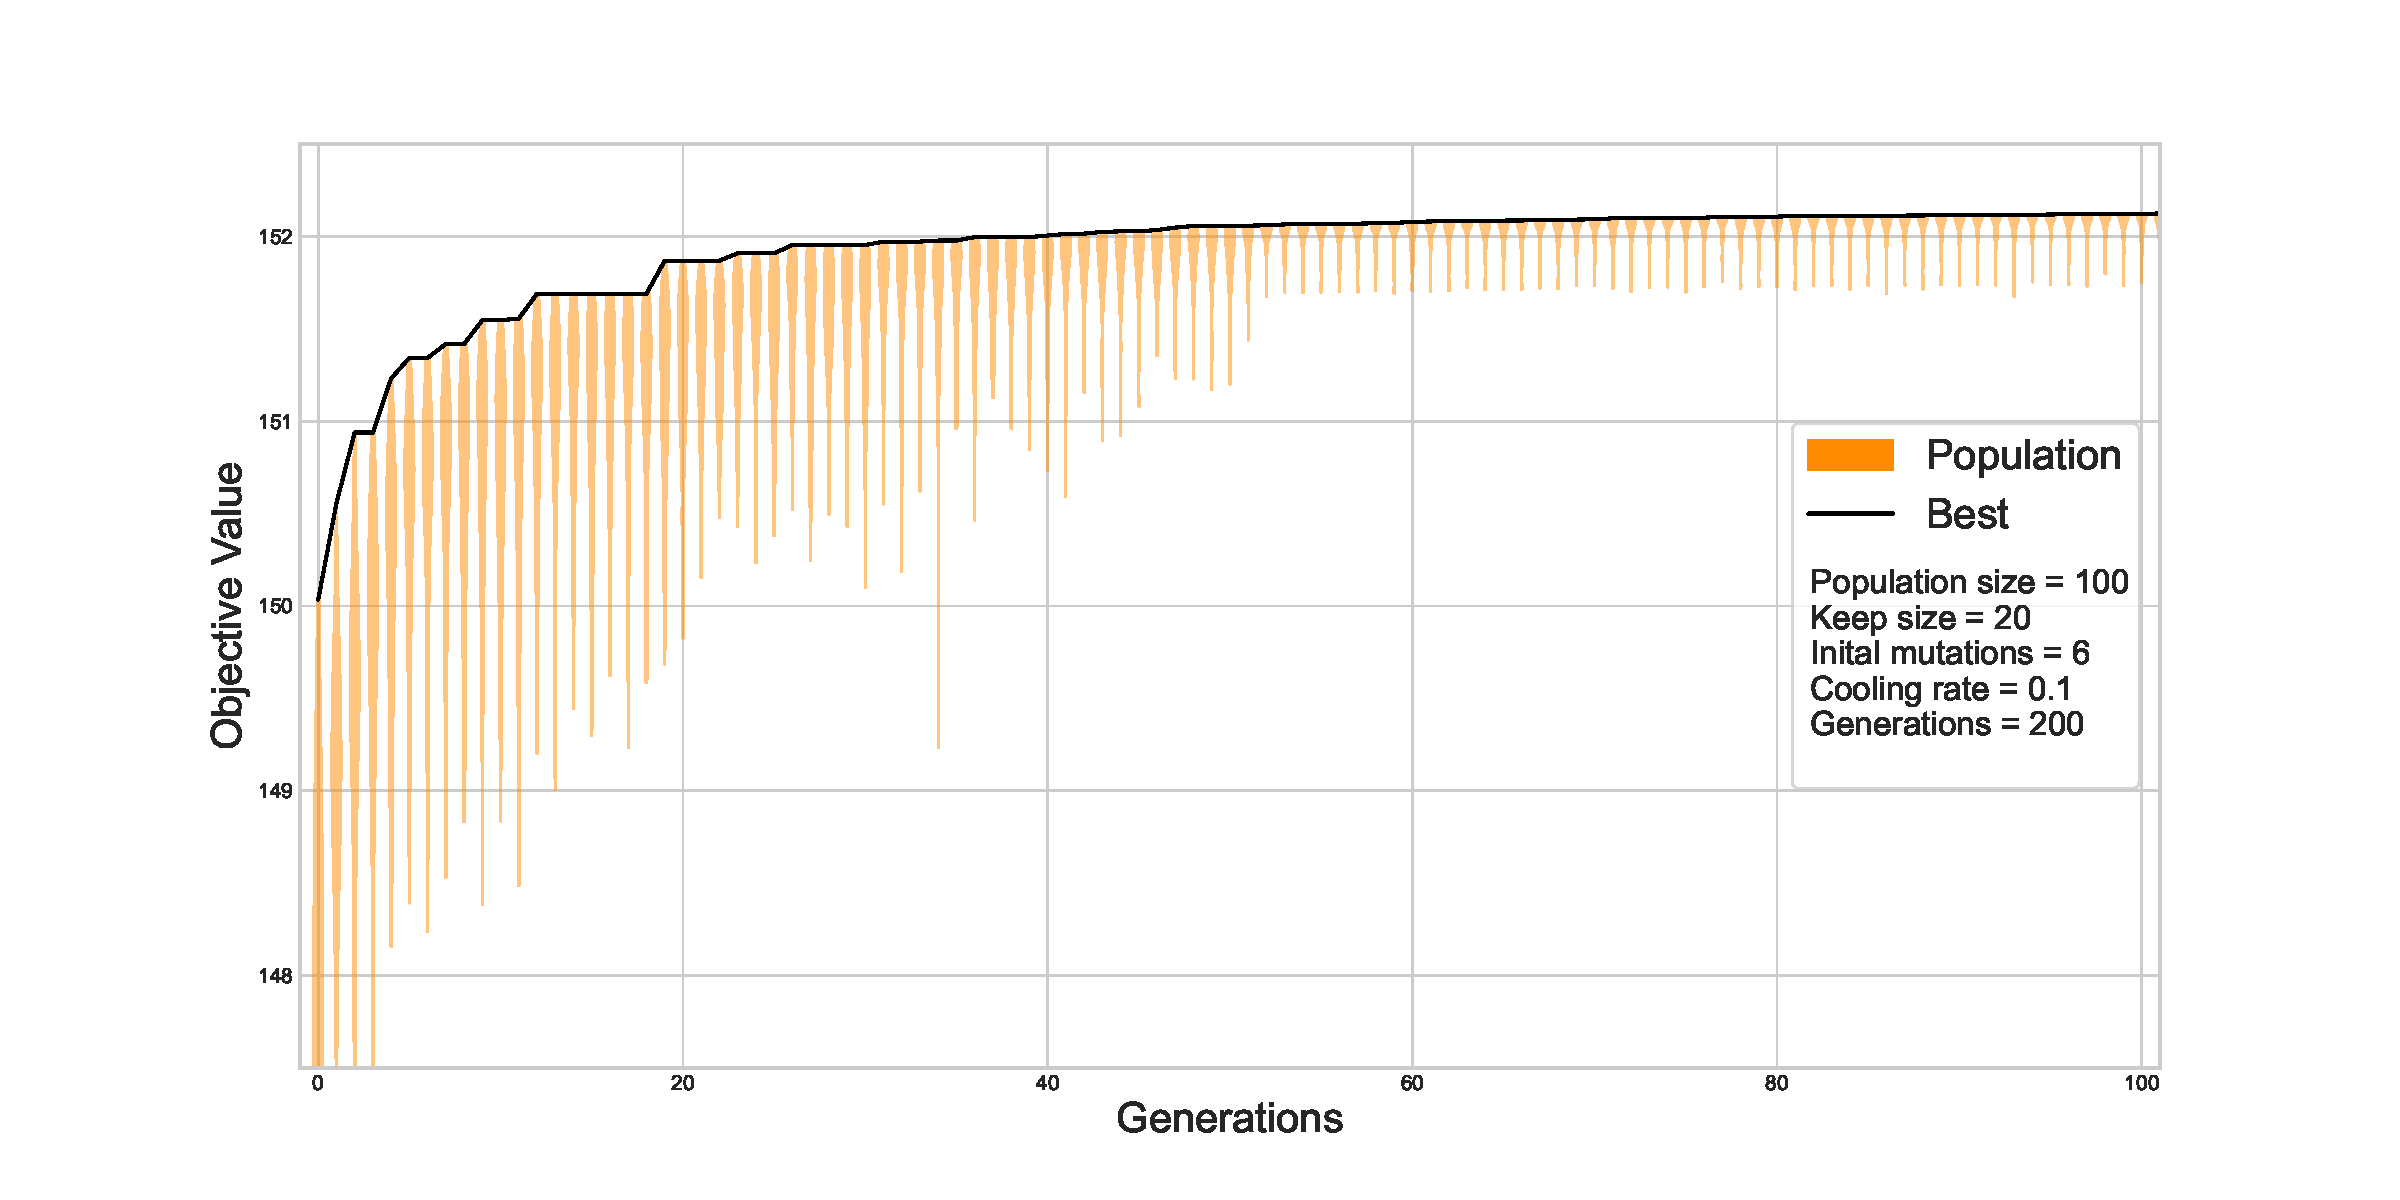
\includegraphics[width=\textwidth]{../images/example-optimisation-run}
\end{center}%
}
\end{frame}

\begin{frame}
\frametitle{Optimised Allocation}
\Wider[4em]{
\resizebox{\textwidth}{!}{%
\begin{tikzpicture}
\draw[draw=none, fill=white] (-7, -4) rectangle (7, 4);
\node at (0, 0)  {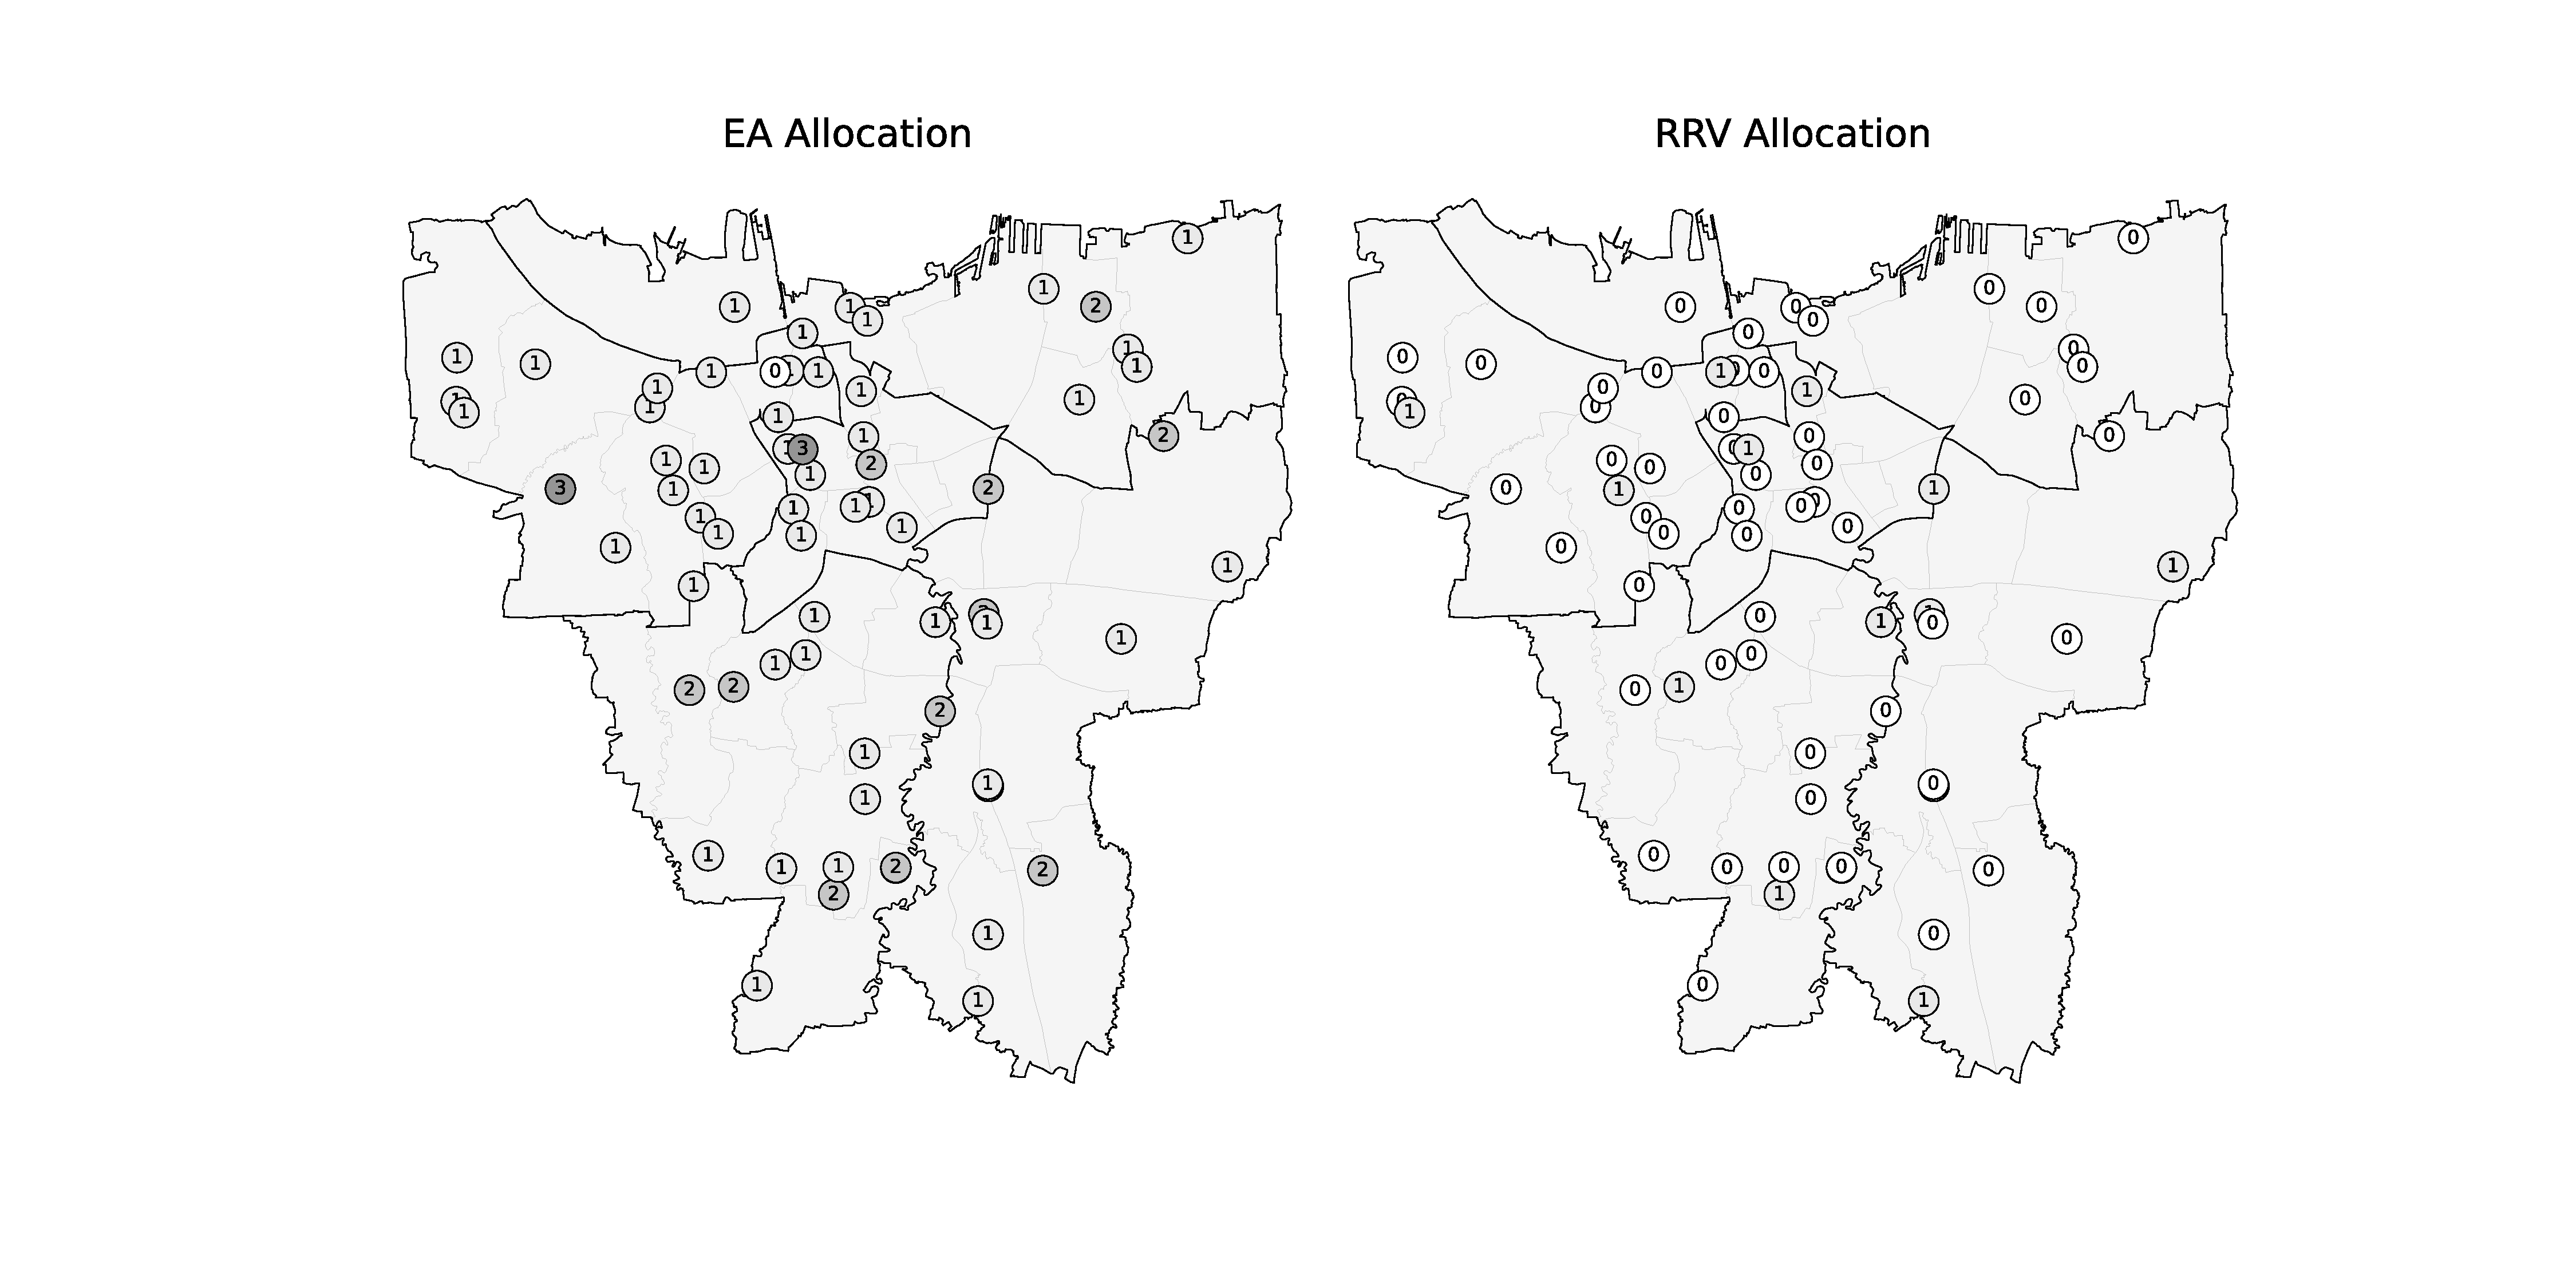
\includegraphics[width=\textwidth]{../images/map_current}};
\end{tikzpicture}%
}%
}
\end{frame}

\begin{frame}
\frametitle{Simulation}
\begin{columns}
\begin{column}{0.4\textwidth}
  \begin{center}
  
\includegraphics[width=0.8\textwidth]{../images/ciwlogo}
  \end{center}
\end{column}
\begin{column}{0.6\textwidth}
\begin{itemize}
  \item Customers are ambulance jobs
  \item Ambulances are servers
  \item Jobs routed to closest ambulance
  \item Sequential logic for secondary vehicles
\end{itemize}
\end{column}
\end{columns}
\end{frame}

\begin{frame}
\frametitle{Simulated Routes}
\begin{center}
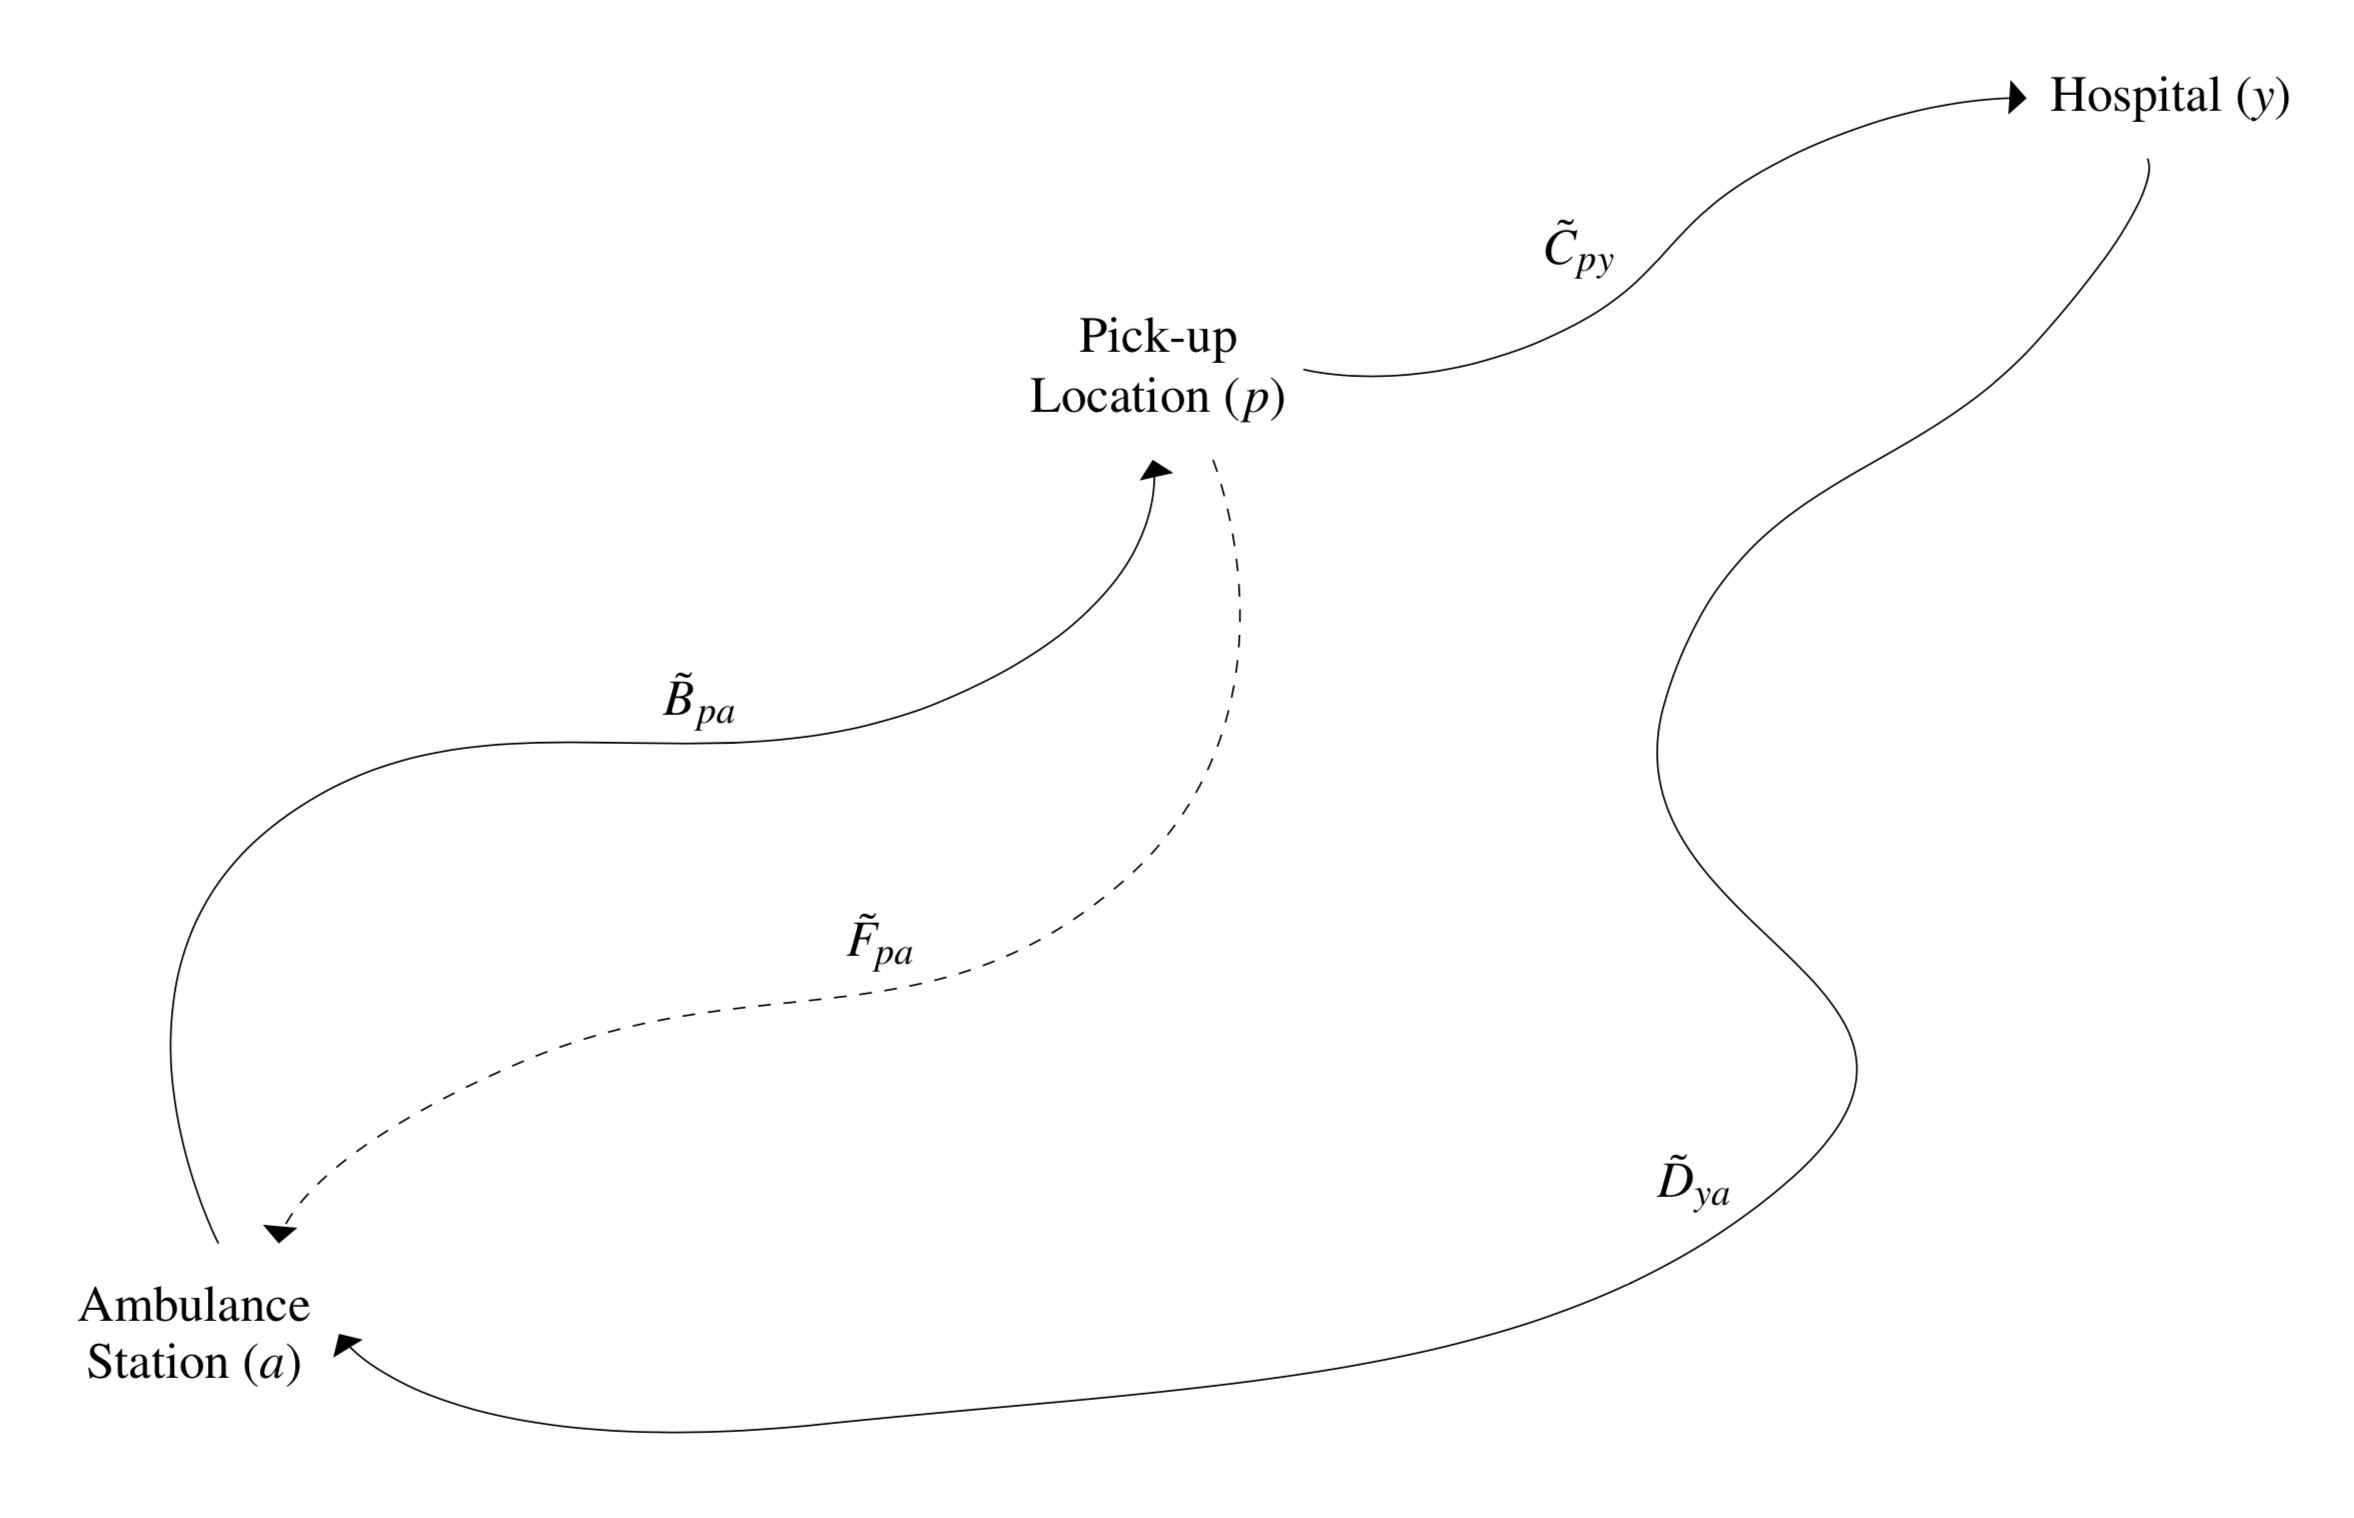
\includegraphics[width=\textwidth]{../images/ambulance_routes}
\end{center}
\end{frame}

% \begin{frame}
% \frametitle{Synchronicity}
% \begin{center}
% 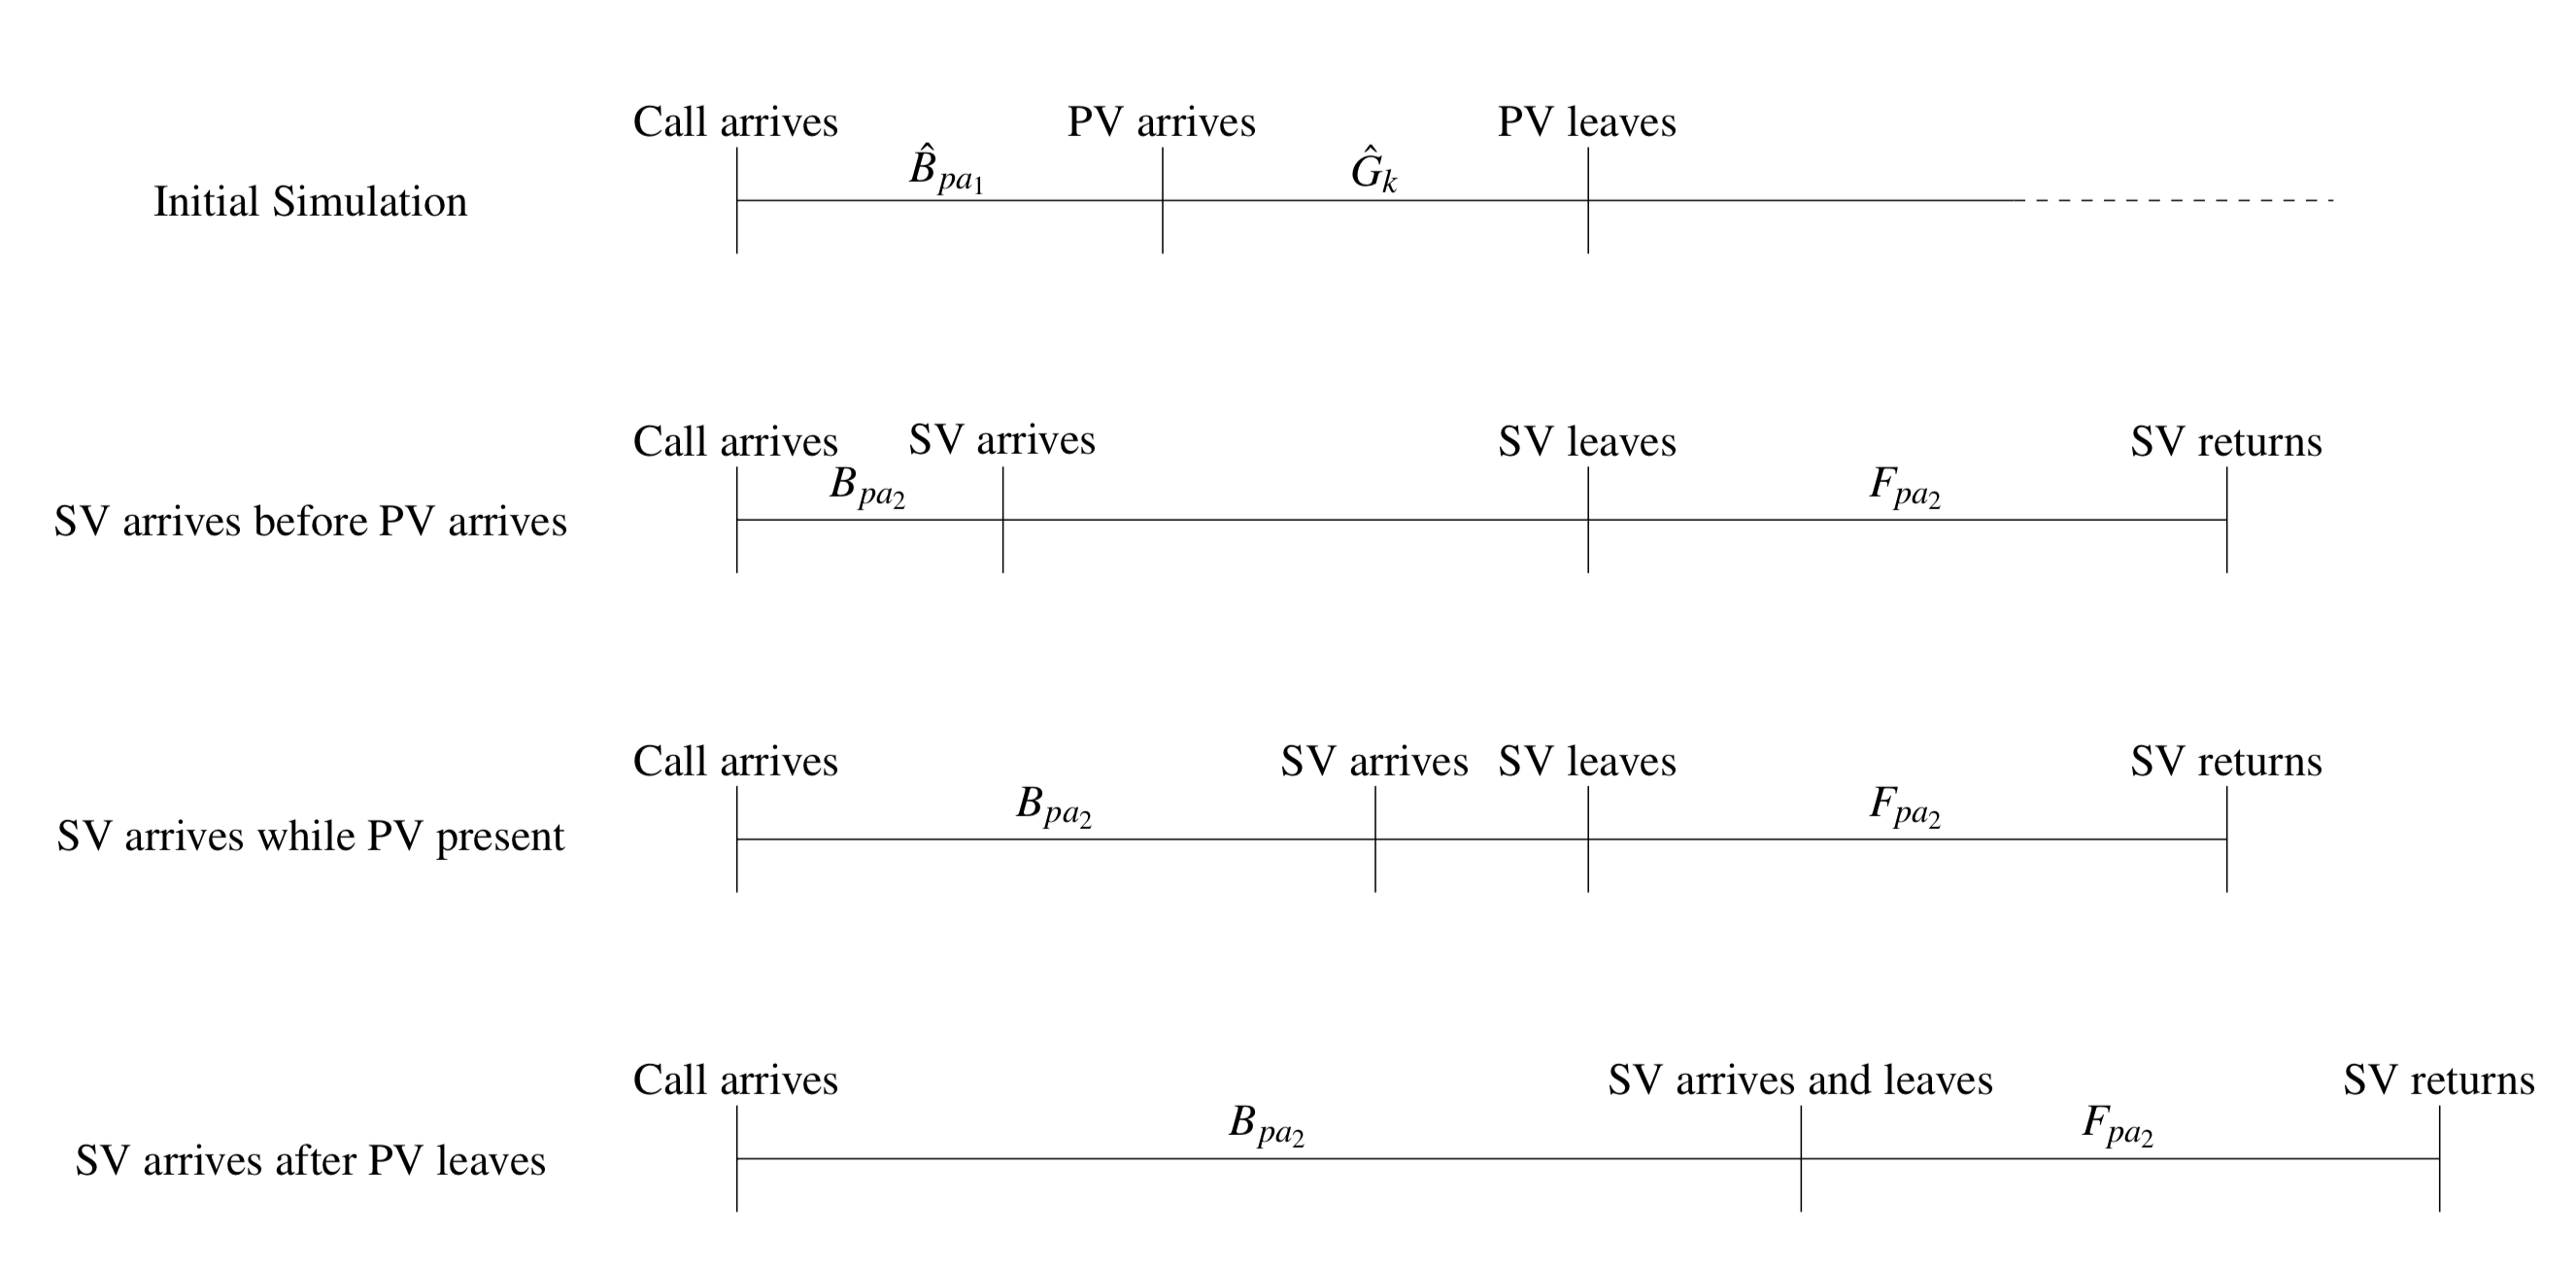
\includegraphics[width=\textwidth]{../images/synchronicity}
% \end{center}
% \end{frame}

\begin{frame}
\frametitle{Current vs Optimised}
\begin{center}
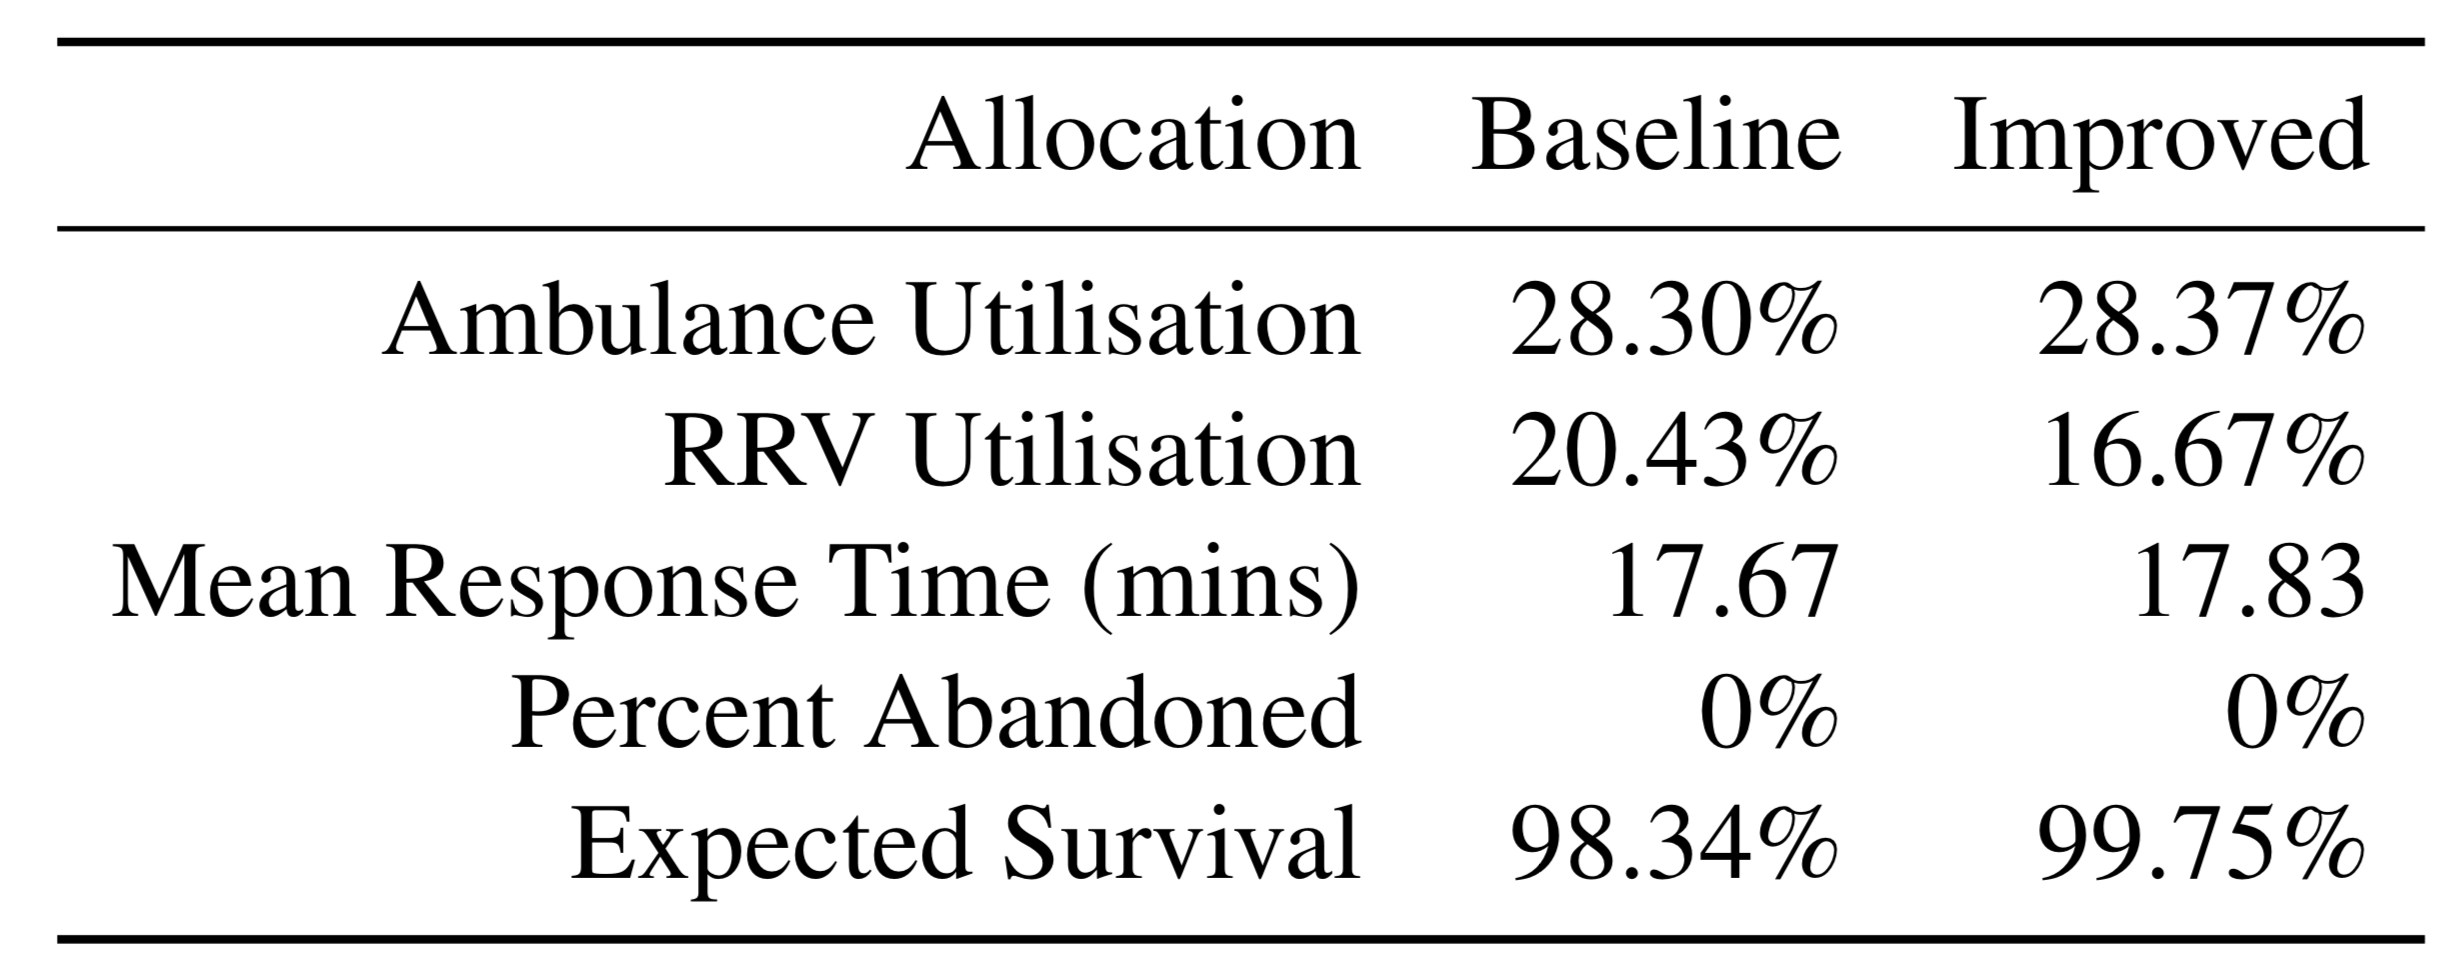
\includegraphics[width=\textwidth]{../images/compare_improved_allocation}
\end{center}
\end{frame}

% \begin{frame}
% \frametitle{Demand Scenarios}
% \begin{columns}
% \begin{column}{0.6\textwidth}
%   \begin{center}
%   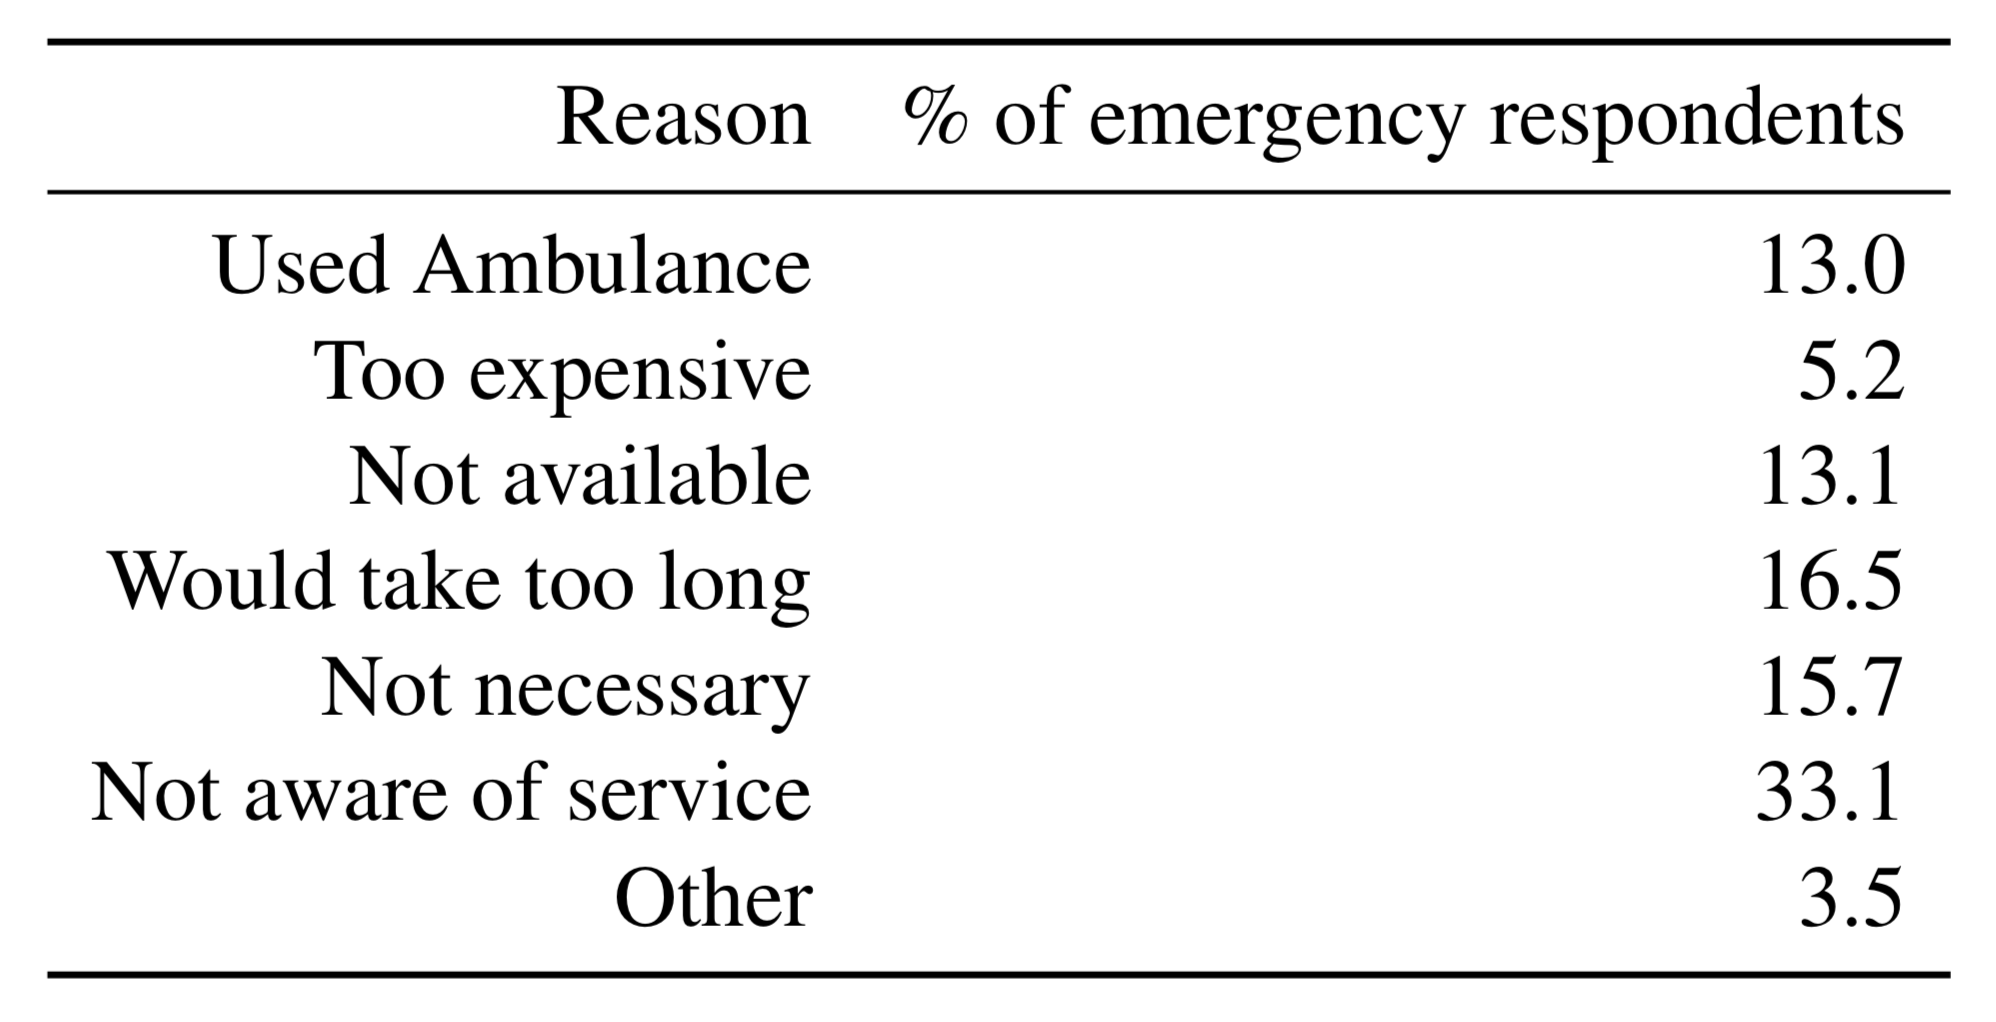
\includegraphics[width=\textwidth]{../images/survey_results}
%   \end{center}
% \end{column}
% \begin{column}{0.4\textwidth}
% \begin{itemize}
%   \item \normalsize{\textbf{\textit{Demand 13}}}\\\footnotesize{Current}
%   \item \normalsize{\textbf{\textit{Demand 19}}}\\\footnotesize{Visibility addressed}
%   \item \normalsize{\textbf{\textit{Demand 34}}}\\\footnotesize{Visibility and reliability addressed}
%   \item \normalsize{\textbf{\textit{Demand 45}}}\\\footnotesize{Visibility, reliability, and cost addressed}
% \end{itemize}
% \end{column}
% \end{columns}
% \end{frame}

% \begin{frame}
% \frametitle{Optimising for Demand Levels}
% \begin{center}
% 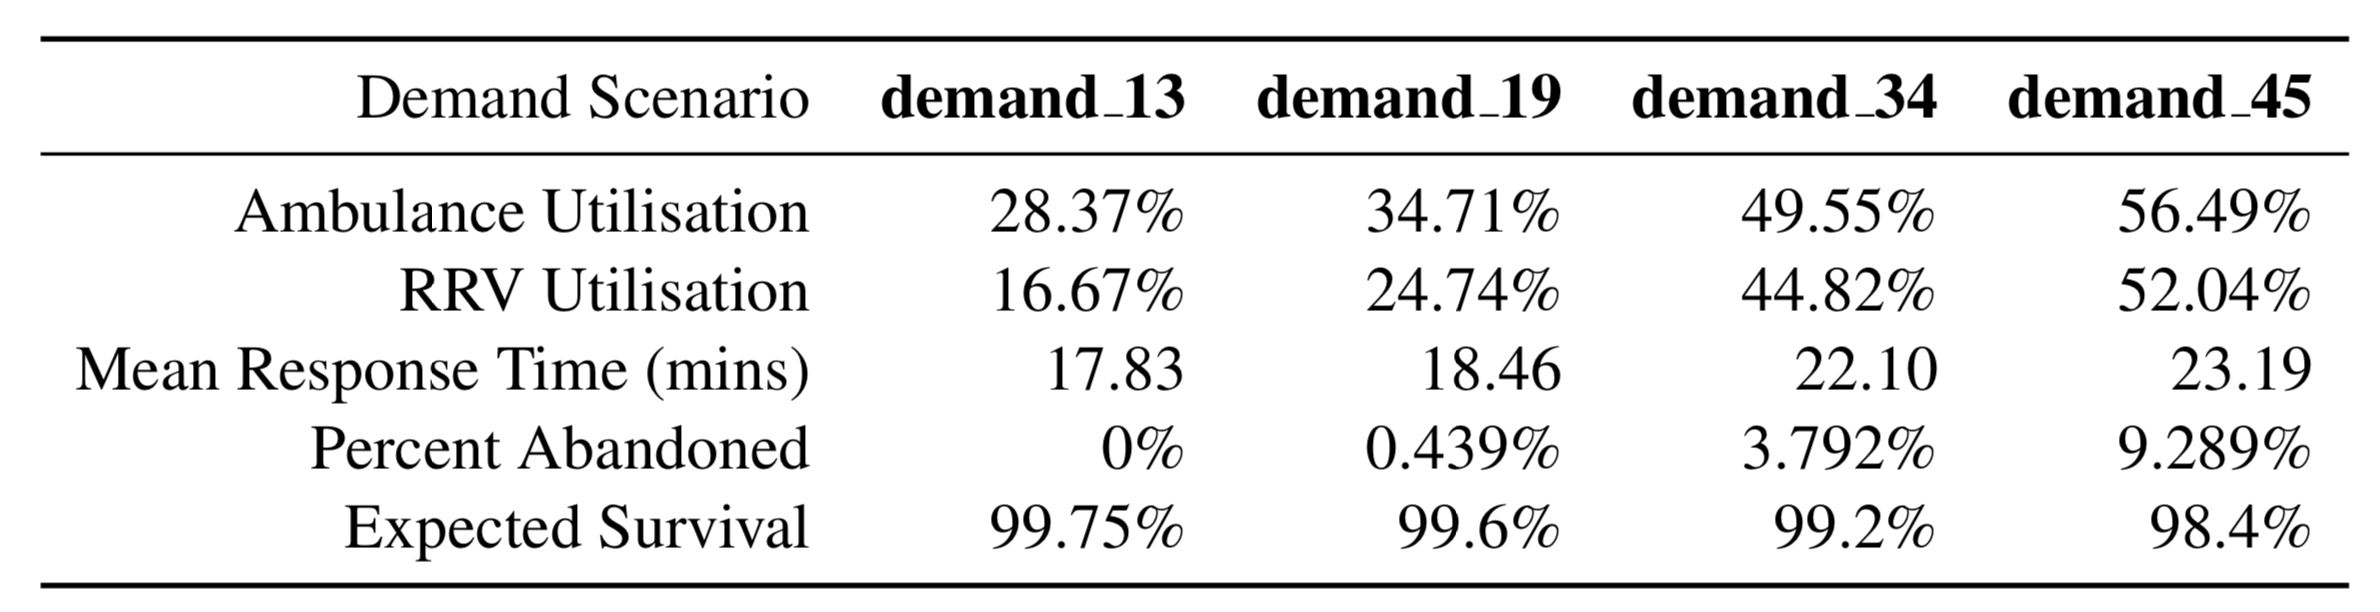
\includegraphics[width=\textwidth]{../images/current_allocation_vary_demand}
% \end{center}
% \end{frame}

\begin{frame}
\frametitle{Summary \& Future Work}
\begin{itemize}
  \item MESLMHPHF objective function
  \item Considers utilisations
  \item Simulation model
\end{itemize}

\rule{\textwidth}{0.5pt}

\begin{itemize}
  \item Consider demand scenarios
  \item Consider vehicle numbers
\end{itemize}

\rule{\textwidth}{0.5pt}

\begin{itemize}
  \item Location dependent $\mu$'s
  \item Replicate work with Welsh Ambulance Trust
\end{itemize}

\end{frame}


\frame{\titlepage}

\end{document}